% ****** Start of file apssamp.tex ******
%
%   This file is part of the APS files in the REVTeX 4.2 distribution.
%   Version 4.2a of REVTeX, December 2014
%
%   Copyright (c) 2014 The American Physical Society.
%
%   See the REVTeX 4 README file for restrictions and more information.
%
% TeX'ing this file requires that you have AMS-LaTeX 2.0 installed
% as well as the rest of the prerequisites for REVTeX 4.2
%
% See the REVTeX 4 README file
% It also requires running BibTeX. The commands are as follows:
%
%  1)  latex apssamp.tex
%  2)  bibtex apssamp
%  3)  latex apssamp.tex
%  4)  latex apssamp.tex
%
\documentclass[%
 reprint,
%superscriptaddress,
%groupedaddress,
%unsortedaddress,
%runinaddress,
%frontmatterverbose, 
%preprint,
%preprintnumbers,
%nofootinbib,
%nobibnotes,
%bibnotes,
 amsmath,amssymb,
 aps,
%pra,
%prb,
%rmp,
%prstab,
%prstper,
%floatfix,
]{revtex4-2}

\usepackage{graphicx}% Include figure files
\usepackage{dcolumn}% Align table columns on decimal point
\usepackage{bm}% bold math
\usepackage{url}
\usepackage{algorithm}
\usepackage{algpseudocode}
%\usepackage{hyperref}% add hypertext capabilities
%\usepackage[mathlines]{lineno}% Enable numbering of text and display math
%\linenumbers\relax % Commence numbering lines

%\usepackage[showframe,%Uncomment any one of the following lines to test 
%%scale=0.7, marginratio={1:1, 2:3}, ignoreall,% default settings
%%text={7in,10in},centering,
%%margin=1.5in,
%%total={6.5in,8.75in}, top=1.2in, left=0.9in, includefoot,
%%height=10in,a5paper,hmargin={3cm,0.8in},
%]{geometry}

\begin{document}

\preprint{APS/123-QED}

\title{Constructing Non-Linear Cosmological Tension Coordinate with Neural Networks}
% \thanks{A footnote to the article title}%

\author{Candidate Number: 8260Q}


\date{\today}

\begin{abstract}
Tensions in cosmology, such as the Hubble tension and the weak lensing $\Omega_m$ - $\sigma_8$ tension, are rising as measurement precision has improved over recent years. We develop the idea of a one-dimensional coordinate which maximises tension between two cosmological datasets. We use a simple neural network with a single hidden layer to represent a non-linear function of cosmological parameters, whose output is the 1D \textit{tension coordinate}. We apply this method to the \textit{Planck} and DES datasets on the following parameters: baryon density $\Omega_b h^2$, matter density $\Omega_m$, Hubble constant $H_0$, optical depth to reionisation $\tau$, matter fluctuation amplitude $\sigma_8$, and scalar spectral index $n_s$. Across all six parameters, we obtain a marginalised Bayes factor of $\log R_t = -16.8 \pm 0.5$, which is equivalent to a non-linear tension of $(5.47 \pm 0.08)\sigma$. Calculating the gradient of the tension coordinate with respect to each parameter, we find the Hubble constant $H_0$ to be the largest contributor to the six-parameter tension. Performing a comparison between parameter pairs using a neural network with two input parameters, we again find the Hubble constant to contain the most tension. This is in contrast to traditional approaches, which usually identifies $\Omega_m$ - $\sigma_8$ to contain the majority of the tension. Interestingly, we find $n_s$ to contribute significantly to the six-parameter tension, but does not contain much tension within itself.

\end{abstract}

%\keywords{Suggested keywords}%Use showkeys class option if keyword
                              %display desired
\maketitle

%\tableofcontents


\section{Introduction} \label{intro}

With cosmological measurements becoming more precise over recent years, disagreements between different datasets and methods have begun to emerge. Observations of parameters surrounding the cosmological constant cold dark matter ($\Lambda \textrm{CDM}$) model have yielded discrepancies, more commonly referred to as \textit{tensions}, of close to $5\sigma$ -- the gold standard of significance in particle physics \cite{Franklin2013}. 

One such tension is the \textit{Hubble tension}. The debate over the Hubble constant's value is one that is hardly new, but in recent years has risen to prominence in cosmology. Disagreement over the Hubble constant began between de Vaucouleurs and Sandage in the 1980s \cite{deVaucouleurs1986, Sandage1975}, and it has now developed into an area of contention between early- and late-universe cosmologists \cite{Planck2020, Abbott2018, Freedman2020, Riess2019, Wong2019}. As it stands, measurements by these two factions are at significant tension of around $5\sigma$ at the most extreme, as shown in Figure \ref{H0_tension}. This has earned the Hubble tension an apt label of a cosmological \textit{crisis}.


\begin{figure}
    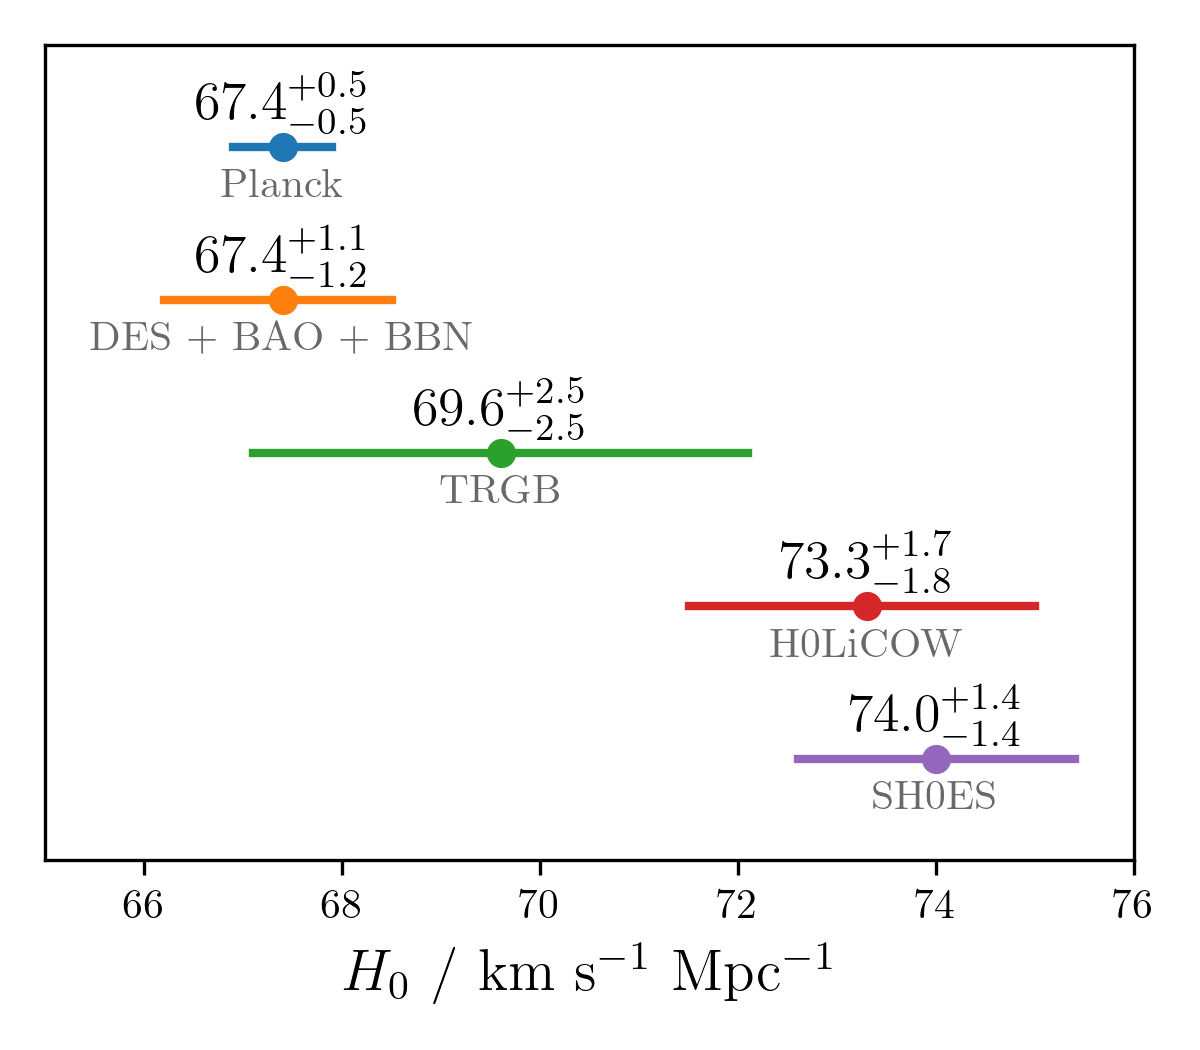
\includegraphics[width=0.8\columnwidth]{../plots/H0 tension.png}
    \centering
    \caption{A compilation of recent measurements of the Hubble constant $H_0$. The top two measurements are from early-universe datasets using $\Lambda$CDM cosmology \cite{Planck2020, Abbott2018}, while the remaining three are from late-universe datasets based off local distance ladder measurements \cite{Freedman2020, Riess2019, Wong2019}. The tension between the \textit{Planck} and SH0ES measurements currently stands at $4.7 \sigma$.}
    \label{H0_tension}
\end{figure}


In addition to the Hubble constant, less severe tensions also exist. Discrepancies of $3\sigma$ have been reported with respect to the matter density $\Omega_m$ and rate of growth of structure $\sigma_8$, between the Cosmic Microwave Background (CMB) data collected by \textit{Planck} and the weak lensing-based Kilo Degree Survey (KiDS) \cite{Heymans2021}. This tension also exist between the \textit{Planck} and the weak lensing-based Dark Energy Survey (DES), which we explore in this paper. Similarly, there has been arguments made for the existence of a ``curvature tension", with inconsistencies of $2.5 \sigma$ to $3 \sigma$ between CMB data alluding to a closed curved universe and the tenet of flat curvature in $\Lambda$CDM cosmology \cite{Handley2021Closed}.

These tensions raise questions surrounding the validity of the well-established, well-tested standard cosmological model -- the $\Lambda$CDM. Are these tensions just an artefact of systematic errors from collecting and analysing datasets? Or do these tensions hint at something more fundamental -- perhaps a modification to the standard model, or more excitingly new physics to take the place of the old one?

However, before we make that leap into the realm of new physics, it is essential for us to examine how tension is quantified. With cosmological datasets being multi-dimensional, the problem of quantifying discrepancies is non-trivial. Datasets that appear to be in mild tension, such as the Dark Energy Survey (DES) Y1 and Planck datasets, have been reported to be consistent when using the canonical Bayes factor $R$ \cite{Handley2019}. This is troubling, and is a reflection of the difficulty of the problem. With tensions likely to increase as measurement precision increases, a variety of tension metrics have been proposed in recent literature \cite{Charnock2017}..

This paper aims to develop the idea of coordinates of maximum tension. With cosmological datasets, larger tensions often exist across multiple parameters rather than within each parameter on its own. A good example would be the $3 \sigma$ tension between $\Omega_m$ and $\sigma_8$ -- the tension is obvious in a two-dimensional plot between these two parameters, but is not as significant when the parameters are inspected individually, as illustrated in Figure \ref{omegam_sigma8}. In a high-dimensional parameter space, it is thus likely that there exists a hidden combination of parameters which exacerbates and maximises tension.

\begin{figure}
    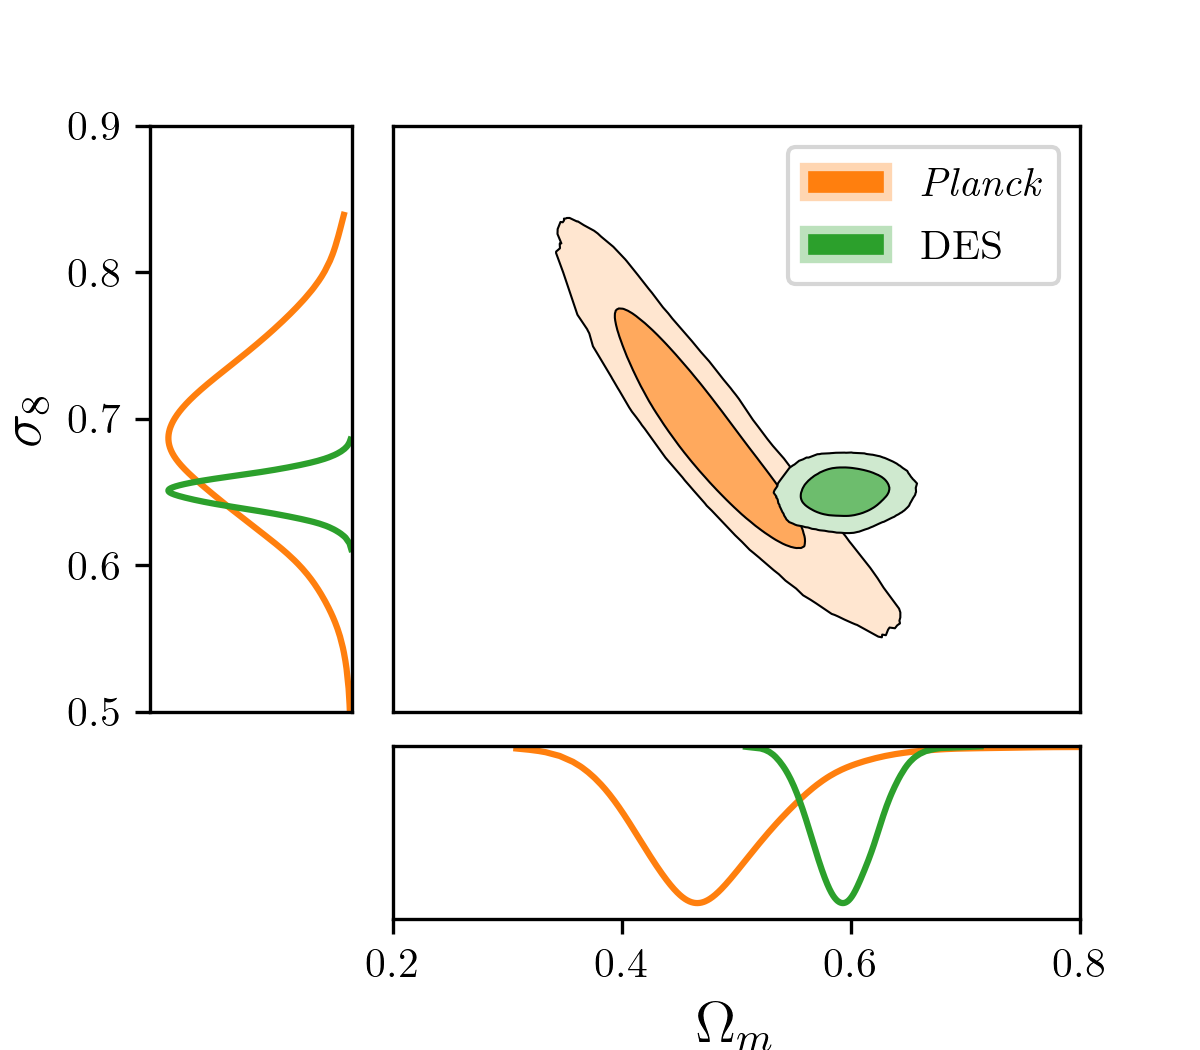
\includegraphics[width=0.9\columnwidth]{../plots/omegam_sigma8.png}
    \centering
    \caption{The main plot shows a two-dimensional marginalised distribution of the \textit{Planck} and DES datasets in the $\Omega_m$ - $\sigma_8$ plane, where the solid contours contain 68\% and 95\% of the marginalised probability mass. The two smaller plots are the one-dimensional marginalised distributions of both datasets in each   parameter.}
    \label{omegam_sigma8}
\end{figure}

In this paper, we explore a non-linear function of parameters for which the marginalised tension is maximised. A neural network is used to achieve this mapping, since the non-Gaussian nature of certain cosmological parameters renders an analytical approach challenging. This tension coordinate is then applied to the \textit{Planck} and DES Y1 datasets. Such an approach could allow us to develop a better intuition of the source of tension, and verify the large tensions that currently exist in $H_0$ and the $\Omega_m$-- $\sigma_8$ plane.



\section{Background}

\subsection{Bayesian Statistics}

We use the following notation of Bayesian statistics, with Bayes' theorem written as
\begin{equation}
    P(\theta|D) = \frac{P(D|\theta)P(\theta)}{P(D)} \, \longrightarrow \, \mathcal{P}_D(\theta) = \frac{\mathcal{L}_D(\theta) \pi(\theta)}{\mathcal{Z}_D}.
\end{equation}
The posterior is denoted as $\mathcal{P}_D$, likelihood as $\mathcal{L}_D$, prior as $\pi$, and evidence as $\mathcal{Z}_D$. Note that the subscript here represents the dataset-dependence of these distributions. 

\subsubsection{Bayesian Evidence}
The Bayesian evidence $\mathcal{Z}_D$ is defined as 
\begin{equation}
    \mathcal{Z}_D = \int \mathcal{L}_D \pi \ \rm{d} \theta.
\end{equation}
Also known as the marginal likelihood in statistical literature \cite{Trotta2008}, the evidence is often deemed to be a natural value for model and dataset comparisons within the Bayesian framework. The calculation of the evidence was historically computationally prohibitive, as it involves a multi-dimensional integral over the entire parameter space. Fortunately, there are now several numerical methods that can reliably estimate the evidence, including thermodynamic integration \cite{Lartillot2006} and nested sampling \cite{Skilling2006, Handley2015}.

\subsubsection{Kullback-Leibler Divergence}

The Kullback-Leibler (KL) divergence $\mathcal{D}_D$ between the prior and posterior is given by
\begin{equation}
    \mathcal{D}_D = \int \mathcal{P}_D (\theta) \log \frac{\mathcal{P}_D (\theta)}{\pi_(\theta)} \ \textrm{d}\theta.
\end{equation}
It describes the information compression between the prior and posterior, and can be interpreted as the average information provided by the posterior. The KL divergence is used later in defining the Suspiciousness statistic, which itself is used to compute a more interpretable tension.

\subsection{Bayes Factor $R$}

The canonical Bayes factor $R$ \cite{Marshall2006} is our tension metric of choice, and forms the basis of our method in this paper. With two datasets $A$ and $B$, the Bayes factor is expressed as
\begin{equation}
    R = \frac{\mathcal{Z}_{AB}}{\mathcal{Z}_A \mathcal{Z}_B}, \quad \rm{with} \ \mathcal{Z}_{AB} = \int \mathcal{L}_A \mathcal{L}_B \pi \ \rm{d}\theta.
\end{equation}
This factor is defined as the ratio between the probability of $A$ and $B$ describing the same parameter space and the probability of $A$ and $B$ describing separate parameter spaces. A value of $R \gg 1$ indicates concordant datasets, and $R \ll 1$ indicates discrepant datasets.

The Bayes factor can be re-expressed as 
\begin{equation}
    R = \int \frac{\mathcal{P}_A \mathcal{P}_B}{\pi} \ \rm{d}\theta.
\end{equation}
This is a more convenient expression to work with, since it sidesteps the numerical complexity of computing evidences. This form of the Bayes factor also makes explicit its prior-dependence, which is arguably a concern \cite{Handley2019}. A broader prior would increase the factor $R$, whilst a narrower prior would reduce $R$ and thus increase tension. Such a dependence means that $R$ is able to hide potential discrepancies with a broad prior. On the other hand, consistent datasets with sensible priors \textit{cannot} be reported to be in tension by the Bayes factor. This means that a value of $R$ indicating tension does in fact point to disagreeing datasets, hence low values of $R$ must be taken more seriously than higher values of $R$.


\subsection{Tension Coordinate}

Many tension quantification methods, including the Bayes factor, have the desirable characteristic of being independent of the choice of parameters and the direction in the parameter space. However, it would also be interesting to be able to describe the spatial structure of the tension, i.e. which parameters contribute most to the tension. As alluded to in the introduction of this paper, it is very probable that there exists a combination of parameters, or more generally a function of the parameter space, which maximises tension between two datasets. The output of such a function is what we call the \textit{tension coordinate}. 

% This coordinate can be expressed as $t = T(\theta)$, where $\theta$ represents the parameter space.

% This idea could be a first step in better understanding the sources of tension between datasets, particularly when one believes there to be more tension than one would expect from a global tension metric.

In this paper, tension is quantified using the Bayes factor $R$. We minimise $R$, calculated in the tension coordinate, to achieve maximum tension. We first demonstrate the tension coordinate for the ideal case of two Gaussian distributions representing two separate datasets. Then, we approach the tension coordinate more practically to tackle non-Gaussian distributions.

\subsubsection{Gaussian example} \label{gaussian_tension}

Let there be two datasets $A$ and $B$ represented by two Gaussian distributions with shared parameters $\theta$. $A$ and $B$ have mean vectors of $\mu_A$ and $\mu_B$, and covariance matrices of $\Sigma_A$ and $\Sigma_B$, respectively. The natural log of the Bayes factor $R$ between these two distributions is written as \cite{Handley2019}
\begin{align}
    \log R &= - \frac{1}{2} (\mu_A - \mu_B)^T (\Sigma_A + \Sigma_B)^{-1} (\mu_A - \mu_B) \\
    &= - \frac{1}{2} \mu^T \Sigma^{-1} \mu
\end{align}
where $\mu = \mu_A - \mu_B$ and $\Sigma = \Sigma_A + \Sigma_B$.

Define the one-dimensional tension coordinate as a linear combination of the parameters, $t = n^T \theta$. The vector $n$ can be naturally described as the direction of maximum tension. To map the Gaussian distributions onto $t$, we marginalise the distributions onto the hyperplanes perpendicular to $n$. This gives a marginalised Bayes factor of
\begin{align}
    \log R_t &= -\frac{1}{2} \big( n^T \mu \big)^T \big( n^T \Sigma n \big)^{-1} \big( n^T \mu \big) \\
    &= -\frac{\big( n^T \mu \big)^2}{2 n^T \Sigma n}.
\end{align}

Minimising $\log R_t$ with respect to $n$, which is equivalent to maximising the marginalised tension, gives the direction of maximum tension as
\begin{equation}
    n \propto \Sigma^{-1} \mu = (\Sigma_A + \Sigma_B)^{-1} (\mu_A - \mu_B).
\end{equation}
Substituting this back into the tension coordinate returns
\begin{equation}
    t = n^T \theta \propto (\mu_A - \mu_B)^T (\Sigma_A + \Sigma_B)^{-1} \theta
\end{equation}
where $t$ is defined up to a normalisation constant.

\subsubsection{Non-Gaussian case} \label{non_gaussian}

Datasets with non-Gaussian distributions bring more complexity to the tension coordinate. Instead of marginalising the distributions onto hyperplanes, it is more general to marginalise the distributions onto hypersurfaces and define a tension coordinate of $t = T(\theta)$. Note that it is not necessary for $t$ to be one-dimensional, but we restrict ourselves to this in this paper. With this definition of the tension coordinate, the marginalised Bayes factor $R_t$ is expressed as
\begin{equation} \label{margin_R}
    R_t = \int \frac{\mathcal{P}_A^{t}(t) \mathcal{P}_B^{t}(t)}{\pi^{t}(t)} \ \textrm{d}t
\end{equation}
where $\mathcal{P}_D^{t}(t) = \int \mathcal{P}_D(\theta) \delta(t - T(\theta)) \ \rm{d}\theta$.

In general, we can define a more practical tension coordinate $t = T(\theta; w)$ described by function parameters $w$. To obtain maximum tension, the function parameters need to be $w = \arg \min_w R_t$. We are free to choose any type of function for $T$, where in the simplest case it can be represented by a linear combination of parameters, as demonstrated in Section \ref{gaussian_tension}. We choose to represent $T$ as a neural network with a single hidden layer, with $w$ as the weights between nodes and $R_t$ as the loss function for gradient descent. A neural network is an appropriate choice given the \textit{universal approximation theorem}, which states that a multilayer feedforward network is able to approximate any bounded continuous function \cite{Hornik1989}. To replicate the simplest case of a linear combination of parameters, we can choose to use a neural network without any hidden layers.


\section{Method}

\subsection{Neural Network and Training}

In this paper, we use a fully-connected neural network with only a single hidden layer with 4096 nodes, as illustrated in Figure \ref{fig:NN}. We find that a single hidden layer is sufficient to fit our maximum tension hypersurfaces around continuous non-Gaussian distributions. The choice of the number of nodes is somewhat arbitrary. Given that this neural network is not used for classification/regression and does not have separate training and testing datasets, we are less concerned with the problem of over-fitting our datasets, hence the large number of nodes. 

\begin{figure}
    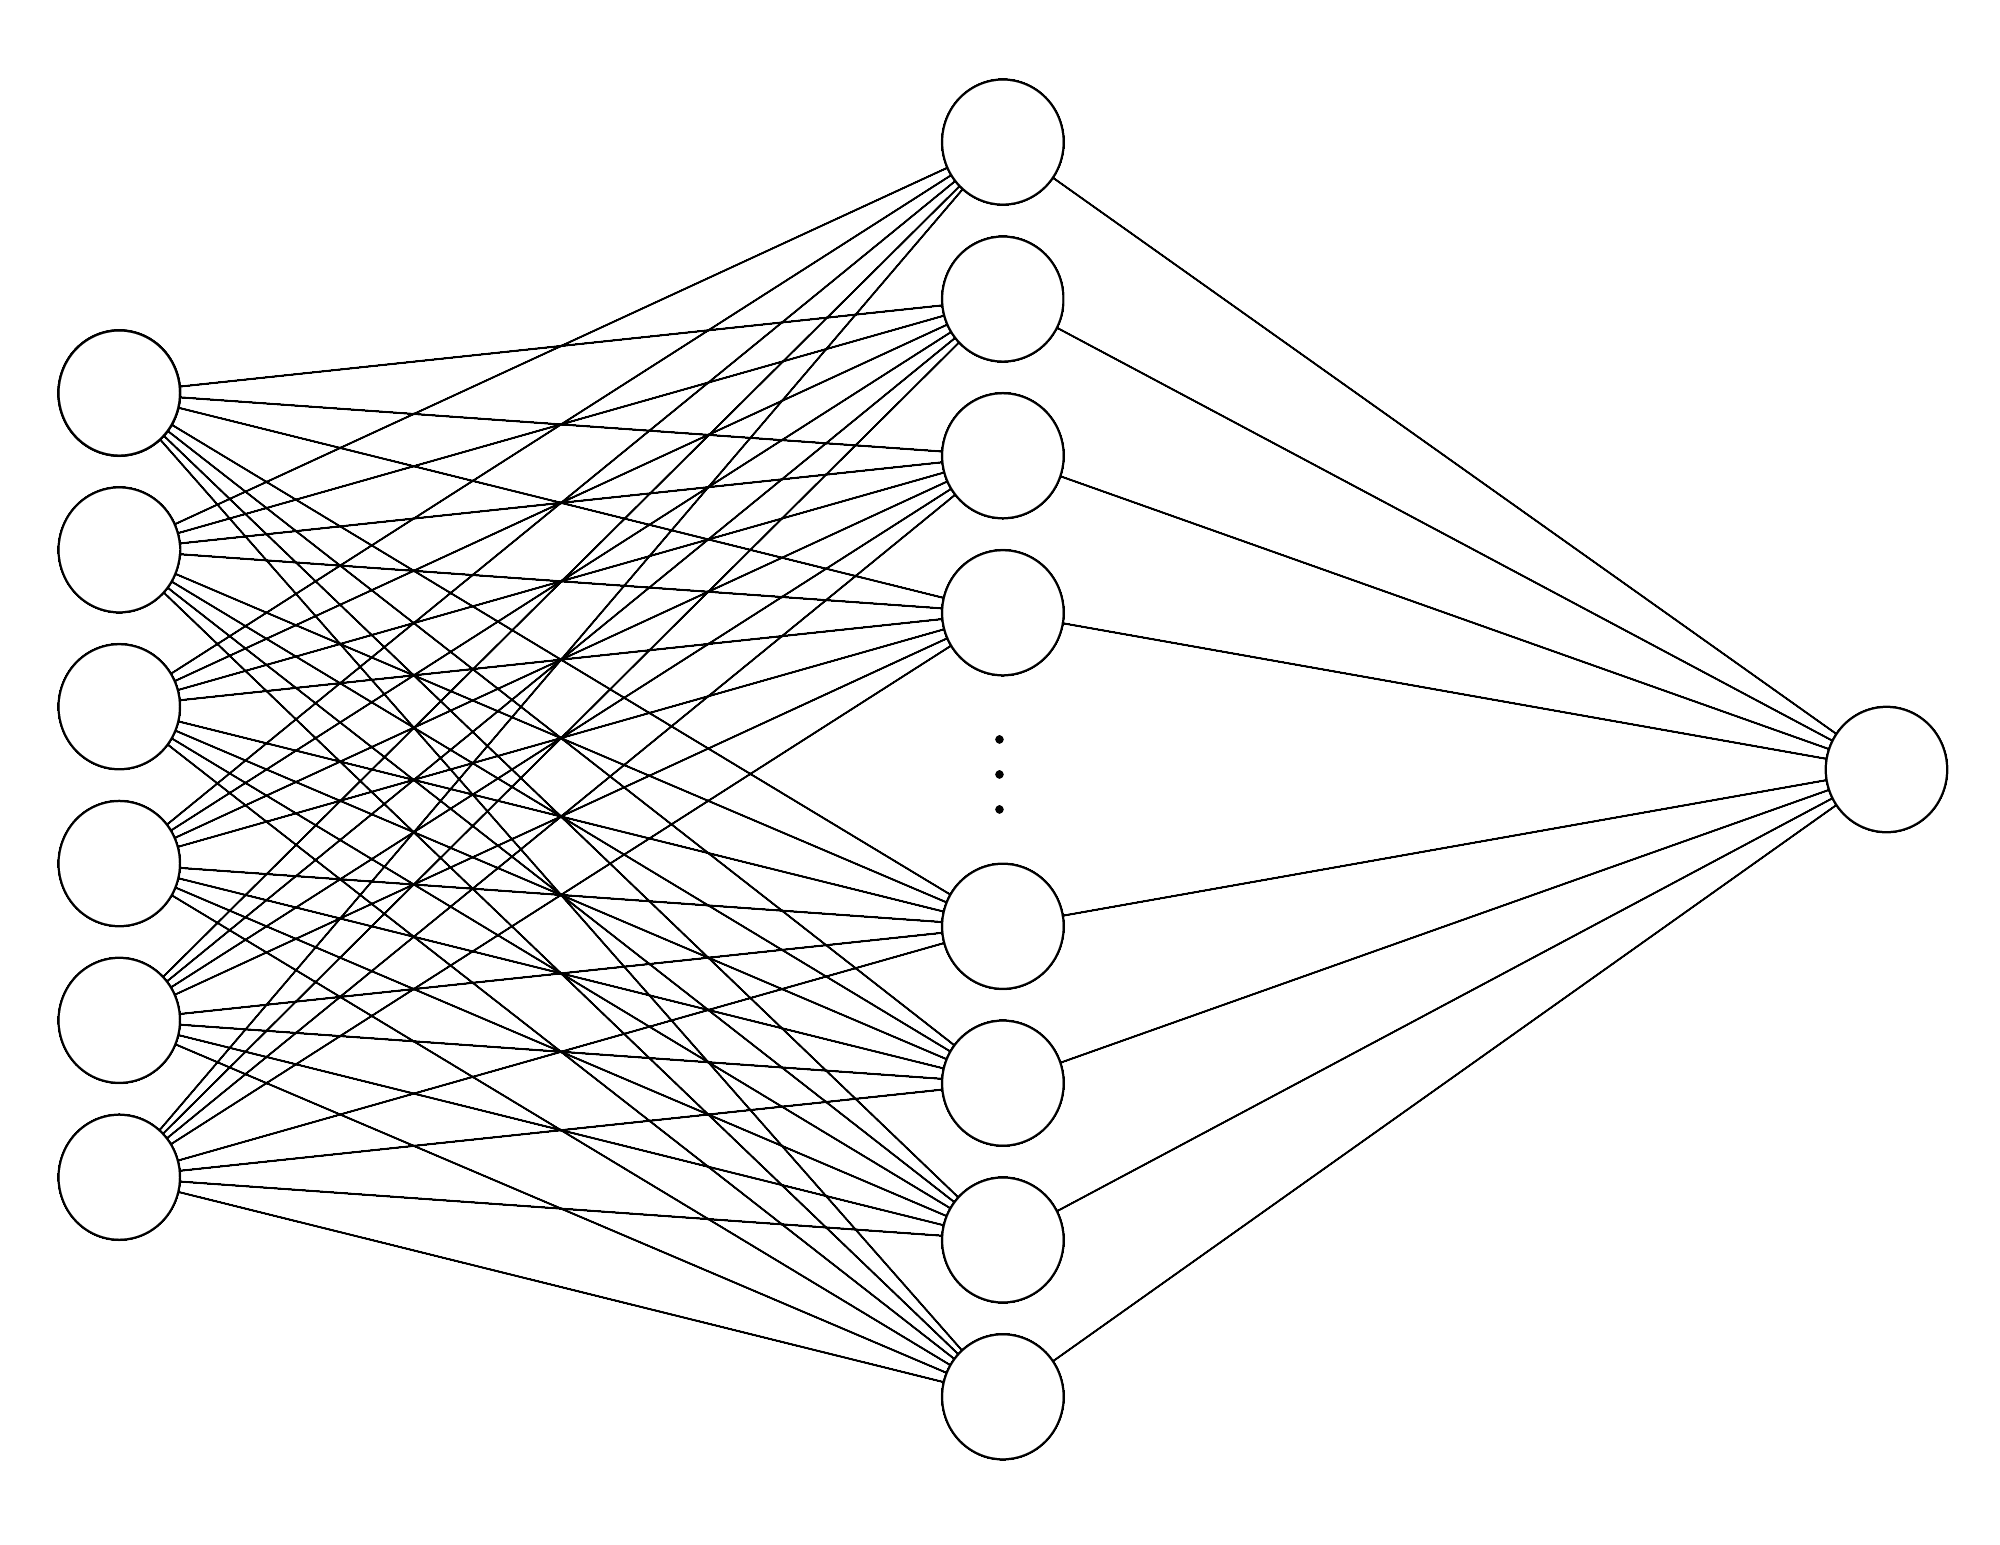
\includegraphics[width=0.8\columnwidth]{images/nn.png}
    \centering
    \caption{A fully-connected neural network with 6 nodes in the input layer, an arbitrary number of nodes in the hidden layer, and a single node in the output layer.}
    \label{fig:NN}
\end{figure}

The inputs to this neural network are the samples from two discrepant datasets with the relevant cosmological parameters, and the output node is the 1D tension coordinate. Due to its popularity and effectiveness in modern deep learning applications \cite{Nwankpa2018}, a rectified linear unit (ReLU) \cite{Nair2010} is chosen as the activation function between the hidden layer and output layer. We can now express our neural network as
\begin{equation}
    t = T(\theta; w) = \sum_i w^{(2)}_i \ \textrm{ReLU} \bigg( \sum_j w^{(1)}_{ij} \theta_j + b_i \bigg)
\end{equation}
where we have cosmological parameters $\theta_{j}$, neural network weights $w^{(l)}_{ij}$, and bias $b_i$. As mentioned in Section \ref{non_gaussian}, the loss function is the Bayes factor calculated in the 1D tension coordinate.

Training this neural network is different from training one for a classification problem. Unlike the 'traditional' method of approximating the gradient using small batches of training data \cite{Keskar2017}, we use all the data points of the two datasets to compute our gradient, and hence calculate the loss function. We do this to provide the Bayes factor, which is our loss function, with a substantial amount of data points to better quantify tension. However, we note that no attempts were made in this paper to experiment with a smaller batch size, e.g. half the data points, thus we cannot confirm that an optimal method was used here. We use the recently popularised Adam optimisation algorithm \cite{Kingma2017} as our stochastic gradient descent method, with an initial learning rate of $10^{-4}$.


\subsection{Numerical Calculation of Bayes Factor} \label{section:numerical_bf}

The calculation of the marginalised Bayes factor $R_t$ forms part of the neural network's optimisation loop. This requires the speed of the numerical computation of $R_t$ to be as rapid and efficient as possible. More importantly, the gradient-based optimisation method chosen necessitates the calculation of $R_t$ to be smooth and differentiable. This rules out the use of binning methods that rely on square top-hat functions. Thus to numerically calculate $R_t$, we rely on a non-parametric smoothing method known as the \textit{kernel density estimator} \cite{Rosenblatt1956, Silverman1986} to estimate the marginalised posteriors and prior in Equation \ref{margin_R}. This method uses (weighted) samples of distributions to makes these approximations.

For an arbitrary one-dimensional weighted dataset $\{(x_{i}, w_{i}), \, i = 1, \dots , n, \, \sum_i^N w_{i} = 1\}$, the kernel density estimator is expressed as
\begin{equation}
    \hat{f}_h (x) = \frac{1}{h} \sum_{i = 1}^{n} w_{i} K \bigg( \frac{x - x_{i}}{h} \bigg)
\end{equation}
where $K$ is the kernel function and $h$ the bandwidth parameter (a notation first introduced by Rosenblatt \cite{Rosenblatt1956}). The kernel function has to satisfy $\int_{\infty}^{\infty} K(x) \, \textrm{d} x = 1$, thus we pick the kernel to be a Gaussian given by
\begin{equation}
    K(x) = \frac{1}{\sqrt{2\pi h^2}} e^{-x^2}.
\end{equation}
Selecting the bandwidth parameter is more complicated. A review of the various choices of bandwidth parameters and bandwidth selection methods can be found in \cite{Turlach1993}. Given our choice of a Gaussian kernel, we choose the general rule of thumb, also known as Scott's rule, as our bandwidth. This rule is written as $h = n_{\textrm{eff}}^{d + 4}$, where $n_{\textrm{eff}} = (\sum w_{i})^2 / {\sum {w_{i}}^2}$ is the effective number of data points and $d$ is the number of dimensions of the distribution being estimated. This setup allows us to effectively approximate unimodal distributions, which the majority of cosmological datasets are.

We use this kernel density estimator to provide an estimate of the marginalised posteriors and the prior found in Equation \ref{margin_R}, which can be denoted by $\hat{\mathcal{P}}_A^{t}$, $\hat{\mathcal{P}}_B^{t}$ and $\hat{\pi}^{t}$ respectively. This gives a marginalised Bayes Factor of
\begin{equation}
    R_t \approx \sum_{j = 1}^{M} \frac{\hat{\mathcal{P}}_A^{t}(t_j) \hat{\mathcal{P}}_B^{t}(t_j)}{\hat{\pi}^{t}(t_j)} \Delta t,
\end{equation}
where we sample the posteriors and prior at points $t_j$ in the 1D tension coordinate at regular intervals, separated by width $\Delta t$.

In practice, it is more effective to use $\log R_t$ instead of $R_t$ as our loss function for the neural network. If we were to use $R_t$, the optimisation steps taken by the neural network becomes increasing small and inconsequential as $R_t \to 0$. On the other hand, $\log R_t$ with its range of $(-\infty, \infty)$ allows gradient descent to make bolder steps towards the local minimum. Taking the natural log of the Bayes factor also prevents underflow issues for extremely discrepant datasets ($R_t \to 0$) by exploiting the LogSumExp method to calculate the posteriors, prior, and ultimately $\log R_t$. The LogSumExp method of calculating a log probability can be found in the source code of \texttt{Scipy}'s \texttt{gaussian\_kde} method \cite{Scipy2020}.

An alternative method to calculating $R_t$ is using a histogram density estimator with a Gaussian envelope rather than a top-hat function \cite{Schutt2017}. However, we find that this method suffers from underflow problems, which undesirably results in $\log R_t \to - \infty$. Hence, we stuck with the Gaussian kernel density estimator.


\subsection{Toy Examples}

We use \texttt{PyTorch} to construct our neural network, and hence also use it to numerical calculate the Bayes factor. Algorithm \ref{algo} takes us through the training of our neural network using \texttt{PyTorch}-esque language. Note that the learning rate of the optimisation method and number of epochs can be adjusted in order to reach a stable local minimum of the Bayes Factor $R_t$.
\begin{algorithm}[H]
\caption{Training of Neural Network}\label{algo}
    \begin{algorithmic}[1]
    \State $X_A \gets $ Dataset A; $w_A \gets $ Weights A 
    \State $X_B \gets $ Dataset B; $w_B \gets $ Weights B
    \State $X_\pi \gets $ Prior; $w_\pi \gets $ Prior Weights
    \State
    \State $net \gets $ NeuralNetwork(in=6, hidden=4096, out=1)
    \State $optim \gets $ AdamOptimizer($net.parameters()$, learning\_rate=$10^{-4}$)
    \State $loss \gets $ LogBayesFactor()
    \State $epochs \gets 500$
    \State
    \For{$i \gets 0$ to $epochs$}
        \State $X_A^t \gets net(X_A)$ \Comment{Tension coordinates}
        \State $X_B^t \gets net(X_B)$
        \State $X_\pi^t \gets net(X_\pi)$
        \State
        \State $R_t \gets loss(X_A^t, X_B^t, X_\pi^t, w_A, w_B, w_p)$
        \State $R_t.backward()$ \Comment{Compute gradients of neural network parameters}
        \State $optim.step()$ \Comment{Make gradient descent step}
    \EndFor
    \State
    \State \textbf{return} $net$
    \end{algorithmic}
\end{algorithm}

Before applying the neural network onto cosmological datasets, we first verify our method using toy datasets. We generate 10000 samples from each of the distributions described below to create our toy datasets.

\begin{figure*}
    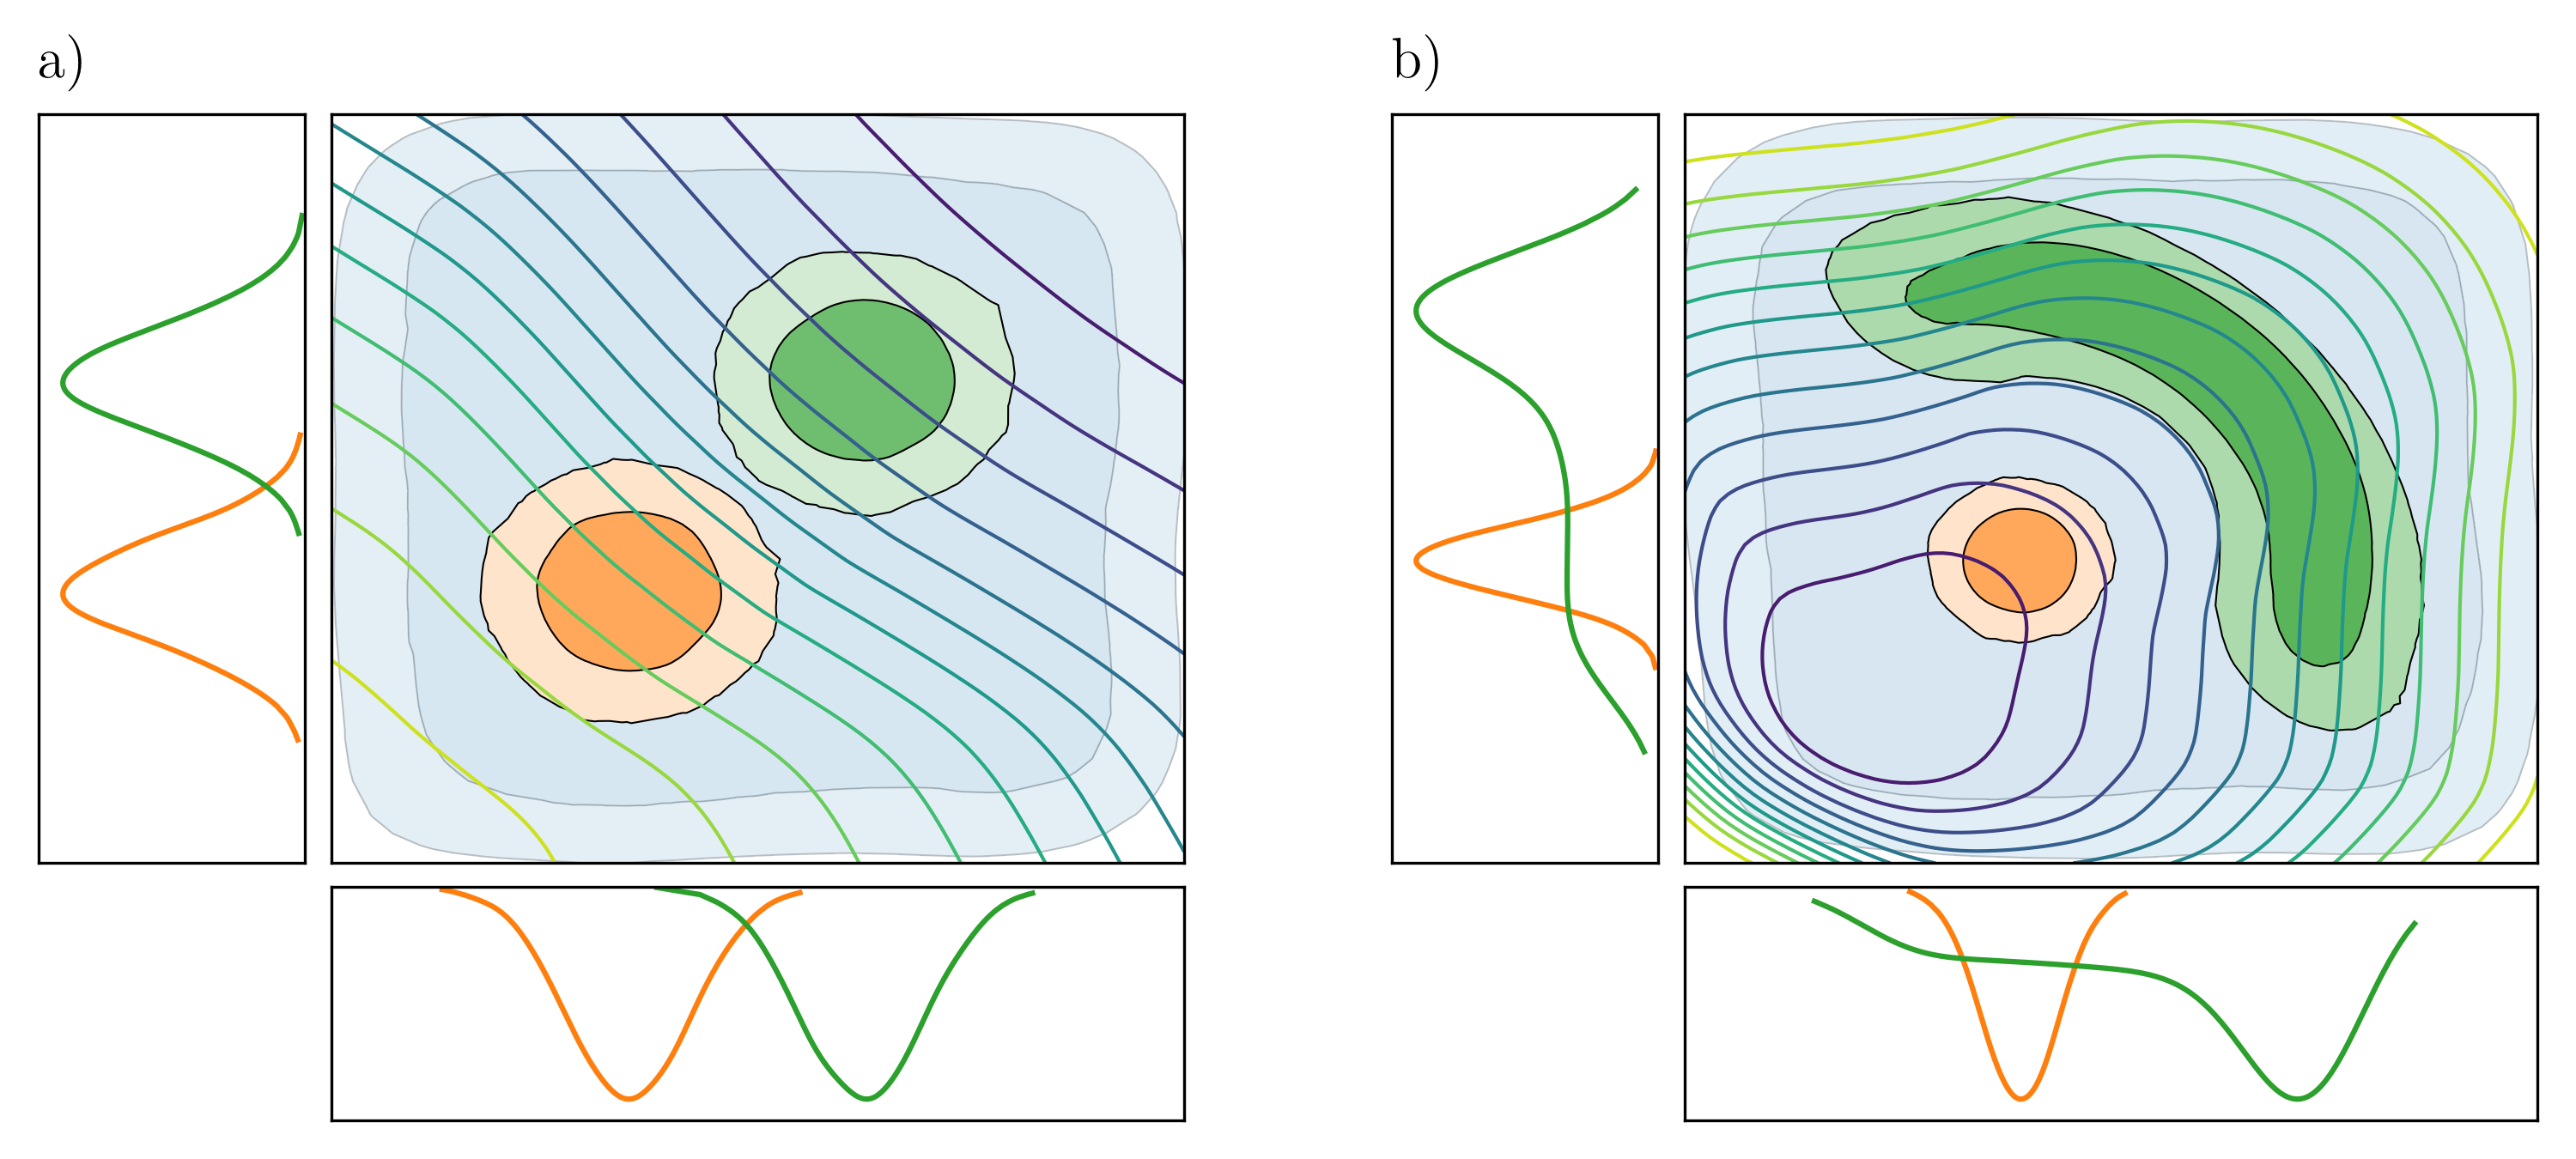
\includegraphics[width=0.9\textwidth]{../plots/toy_wide.png}
    \centering
    \caption{The main contour plots illustrate the iso-tension coordinate hypersurfaces shaped by the neural network after training for 500 epochs on our toy examples. a) shows two Gaussian distributions and b) shows a Gaussian distribution accompanied by a 'banana-shaped' distribution. The faded blue distribution in the background is the prior. The smaller plots along the $x$ and $y$ axes show the marginalised distributions of these toy examples in their respective axes.}
    \label{fig:toy}
\end{figure*}

The very simplest case to begin with would be two discrepant 2D Gaussian distributions, that are also discrepant in each dimension individually. In our example, we place these two distributions around $5\sigma$ apart, and encase them in a square prior, as seen in Figure \ref{fig:toy}(a).  Our neural network is able to fit rough hyperplanes perpendicular to a line connecting the two distributions. This result agrees with the analytical tension coordinate for the Gaussian case derived in Section \ref{gaussian_tension}.

The next example can be seen in Figure \ref{fig:toy}(b). We are still working in two dimensions, but now we have a Gaussian distribution accompanied by a concave quarter-circle distribution. These two distributions are discrepant in two dimensions, but have a considerable overlap in their 1D marginalised distributions. We use this example, albeit an exaggerated example, to reinforce the idea that multi-dimensionality is able to hide non-linear tensions. With this setup, we expect the hypersurfaces, or more simply the contour lines, to be shaped around the 'banana-like' distribution, with directions of maximum tension radiating outwards from the central Gaussian distribution. This is exactly what we see from our results, as illustrated in Figure \ref{fig:toy}(b).

It is crucially important to note that the statistical power of our neural network only lies in the region between our two distributions, and begins to falter as we navigate further away. This effect is obvious in both of our toy examples. In the first case, we see the contour lines bending in the bottom-right and upper-left corners of the plot. In the second example, the curve of the contours do not exactly follow the outer curve of the 'banana-shaped' distribution as we would have expected if the neural network was able to extrapolate well.


\subsection{Cosmological Dataset}

In this paper, we work solely with the cosmological datasets collected by the DES and the \textit{Planck} satellite. We choose these two datasets because of the well reported tensions between them in recent years \cite{Handley2019, Lemos2020}. The tensions mentioned in Section \ref{intro} of this paper, such as the $3\sigma$ tension in the $\Omega_m$ - $\sigma_8$ plane, also exist between these two datasets.

We use the following six cosmological parameters -- baryon density $\Omega_b h^2$, matter density parameter $\Omega_m$, Hubble constant $H_0$, optical depth to reionisation $\tau$, matter fluctuation amplitude $\sigma_8$, and scalar spectral index $n_s$. The derived parameters of $\Omega_m$, $H_0$ and $\sigma_8$ are chosen over the three other independent cosmological parameters of dark matter density $\Omega_c h^2$, angular acoustic scale $100 \theta_*$ and log of primordial fluctuation amplitude $\log A_s$,  because tensions in these derived parameters are well-known. Applying our neural network to these parameters with established discrepancies allows us to verify and reinforce the existing tension in them.

We obtain the DES Y1 and \textit{Planck} datasets from \cite{Dataset}, and use the prior from the DES dataset as the shared prior. This source provides nested sampling chains for all of the independent, derived and nuisance parameters of both datasets. We use the \texttt{anesthetic} \texttt{Python} library \cite{anesthetic} to extract weighted samples from the nested sampling chains. We normalise the datasets such that the DES and \textit{Planck} posteriors lie in the range of $[0, 1]$ for the six parameters. This normalisation allows our neural network to learn and converge faster to a minimum.


\subsection{Identifying the Source(s) of Tension} \label{section:source}

\subsubsection{Six Parameters}

We first train our neural network on all six cosmological parameters to produce a 1D tension coordinate. This gives us an initial intuition of the maximum tension that can be formed between the DES and \textit{Planck} posteriors in these six parameters. To evaluate the contribution of each parameter to the tension, we calculate the derivative of the 1D tension coordinate $t$ with respect to the six parameters. Performing a Taylor expansion on $t$
\begin{equation}
    t = t_0 + \Delta \theta \nabla t + \mathcal{O}((\Delta \theta)^2),
\end{equation}
we would expect a parameter with a larger absolute gradient to be more influential in defining the tension coordinate, hence contributing more to the tension. It is important to remind ourselves that our DES and \textit{Planck} posteriors have been normalised to a range of [0, 1], hence such a comparison of gradients is fair.

\subsubsection{Pair-wise Comparison}

To verify our results from training our neural network on all six parameters, we make pair-wise comparisons between the six cosmological parameters. We construct separate neural networks with two input nodes for each of the fifteen combinations of parameter pairs. This allows us to rank parameter pairings in terms of their contribution to the discrepancy between the two posteriors. This will also enable us to identify parameters containing the most/least tension, and compare the results obtained via this method with the method of calculating gradients from the six-parameter tension.


\subsection{Standardising the Tension Coordinate}

Performing training repetitions on the same neural network architecture with identical data samples often yields 1D tension coordinates with varying ranges. This happens because of the many local minima in the loss function landscape. This renders comparison between training runs difficult. It is thus important to transform the tension coordinate to one that is standardised.

We transform the coordinate to one where the prior is uniform and flat. To perform this transformation, we use the cumulative distribution function of the marginalised prior, which we denote as $\Pi^t(t) = \pi^t(X_\pi^t < t)$, to transform the posteriors and priors such that $\hat{\pi}^{t'}_P = \Pi(X_\pi^t)$, $\hat{\mathcal{P}}_A^{t'} = \Pi(X_A^t)$ and $\mathcal{P}_B^{t'} = \Pi(X_B^t)$. This gives a consistent range of $[0, 1]$ for the transformed 1D tension coordinate $t'$. We will drop the prime from here on, and let $t$ refer to the transformed coordinate. Note that this transformation does not affect the marginalised Bayes Factor $R_t$ or the calculation of tensions.


\subsection{Computing a More Interpretable Tension}

The marginalised Bayes factor is a good method to identify tension. However, it is arguably less interpretable compared to using $\sigma$. To get from the output of the neural network to a $\sigma$ value, we follow the steps detailed in \cite{Handley2021}.

We first compute the Suspiciousness statistic $S_t$ between the two posteriors, which is expressed as
\begin{equation}
    S_t = \frac{R_t}{I_t}, \quad \textrm{where } I_t = \frac{\mathcal{D}_A \mathcal{D}_B}{\mathcal{D}_{AB}}.
\end{equation} 
The subscript $t$ reiterates that we are working in the 1D tension coordinate. The numerical calculation of $S_t$ can be done in a very similar manner to the marginalised Bayes factor $R_t$ using kernel density estimators, as described in Section \ref{section:numerical_bf}. We may then approximate our two posteriors in the 1D tension coordinate with a Gaussian (which is a reasonable assumption, given Figure \ref{fig:six_compare}), and arrive at an expression of 
\begin{align}
    \log S &= \frac{d}{2} - \frac{\chi^2}{2}, \\
    \chi^2 &= (\mu_A - \mu_B)(\Sigma_A + \Sigma_B)^{-1}(\mu_A - \mu_B),
\end{align}
where $d$ is the Bayesian combined model dimensionality \cite{Handley2019} of the two datasets, and  $\mu_D$\ and $\Sigma_D$ are the means and covariances of the two marginalised posteriors. $\chi^2$ here follows a chi-squared distribution. This is all derived in \cite{Handley2019}.

We can obtain a $p$ value via the probability density function of the chi-squared distribution
\begin{equation}
    p = \int_{d - 2 \log S}^{\infty} \frac{x^{d/2 - 1} e^{-x/2}}{s^{d/2} \Gamma(d/2)} \ \textrm{d} x
\end{equation}
and convert this to a $\sigma$ value using the inverse error function
\begin{equation}
    \sigma (p) = \sqrt{2} \textrm{erf}^{-1} (1 - p).
\end{equation}
The final conversion is possible because we approximate the marginalised posteriors as Gaussians.

We choose to use a value of $d \approx 4$ for the DES and \textit{Planck} datasets, as calculated in \cite{Handley2019}, since we source our data from the same paper \cite{Dataset}.



\section{Results and Discussion}

\subsection{Six Parameters} \label{section:six}

We train our neural network for 500 epochs, starting off with a learning rate of $10^{-4}$ for our Adam optimiser and dropping to $10^{-5}$ as we approach $\log R_t \approx -8$. We find that this setup gives a quick and somewhat stable gradient descent. Knowing that neural networks are only able to optimise to a local minimum rather than the global minimum, we perform 10 training repetitions to give a rough estimate of the lowest possible marginalised Bayes factor. 

The results from the 10 training runs are detailed in Table \ref{table:six_params}, and accompanied by the tension calculated from the coordinate derived from the Gaussian assumption from Section \ref{gaussian_tension}. The significant difference between theses two values gives an initial impression of the neural network's ability to identify a tension coordinate which maximises tension. The density plots of the marginalised posteriors drawn in Figure \ref{fig:six_compare} further demonstrates how the neural network is able to uncover the discrepancy between the two datasets, bringing the tension to beyond $5\sigma$.

\begin{table}
    \begin{ruledtabular}
    \begin{tabular}{lrr}
         & Gaussian assumption & Neural network \\
        \colrule
        $\log R_t$ & $-0.9$ & $-16.8 \pm 0.5$ \\
        $\log S_t$ & $-2.4$ & $-17.9 \pm 0.5$ \\
        $p$ value & $6.6\%$ & $(4.6 \pm 2.2) \times 10^{-6}\% $ \\
        tension & $1.84\sigma$ & $(5.47 \pm 0.08)\sigma$ \\
    \end{tabular}
    \end{ruledtabular}
    \caption{The quantities related to the six-parameter tension calculated in a 1D tension coordinate obtained using two different methods -- the Gaussian assumption detailed in Section \ref{gaussian_tension}, and our neural network with six input nodes. No errors are given for the Gaussian assumption case because the tension coordinate can be constructed analytically.}
    \label{table:six_params}
\end{table}

\begin{figure}
    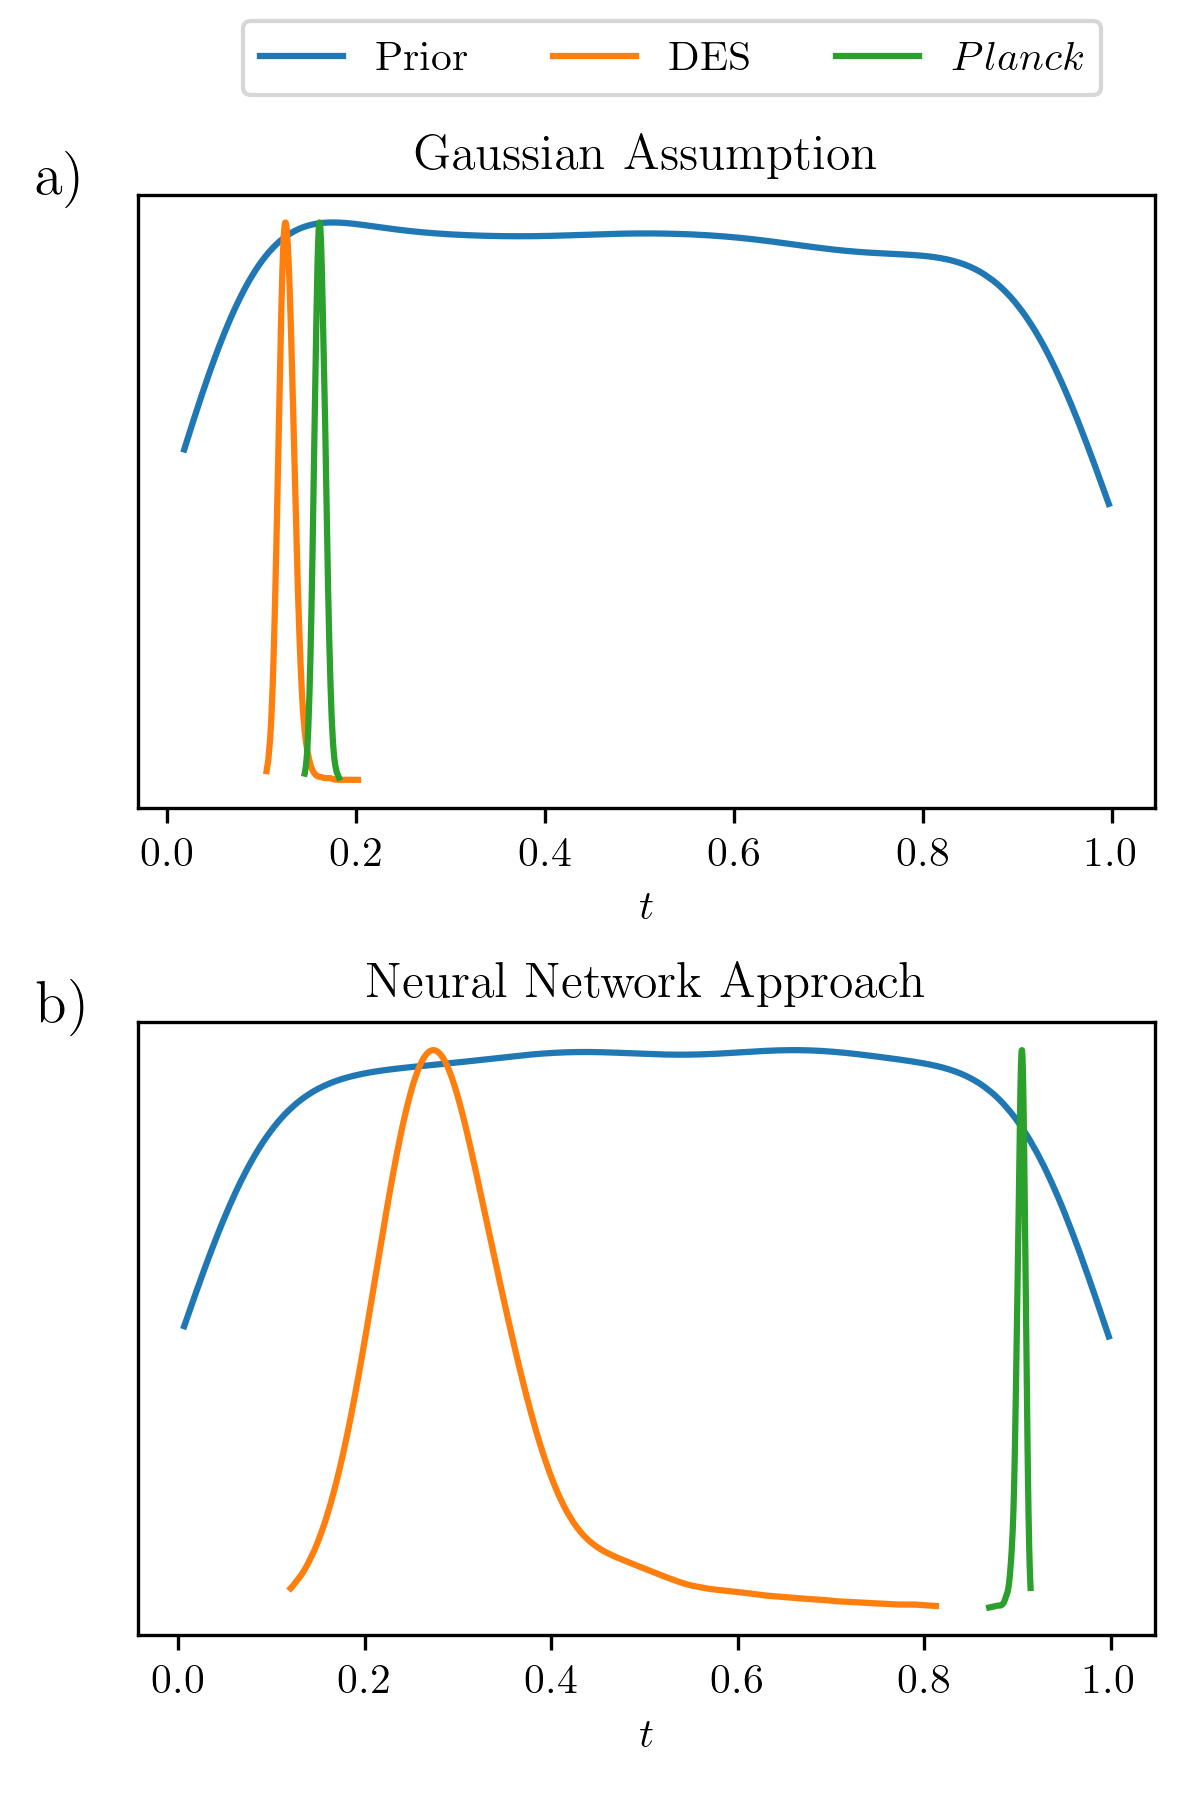
\includegraphics[width=0.8\columnwidth]{../plots/six_1d_compare.png}
    \centering
    \caption{Density plots of the marginalised posteriors of the DES and Planck datasets, and the prior, in the 1D tension coordinate. (a) uses the Gaussian assumption described in Section \ref{gaussian_tension} and (b) uses the neural network approach. Note that the prior is uniform across the range of the tension coordinate, and the bend at the edges of the prior is an just artefact of the kernel density estimator method.}
    \label{fig:six_compare}
\end{figure}

The neural network's effectiveness in capturing the non-linearity of the tension between the two datasets is illustrated in Figure \ref{fig:six}. In these 2D marginalised plots, we observe how our method is able to carve out hypersurface contours isolating the narrower posterior of the \textit{Planck} dataset. For some of the plots, including the $\Omega_b h^2$ - $\tau$ and $\sigma_8$ - $\tau$ plots, the contours go to the extent of encircling the \textit{Planck} posterior. The plots between the tension coordinate and cosmological parameters in the final row of the same figure also begin to describe the contribution of each parameter to the six-parameter tension. However, the wide constraints of the DES dataset renders an analysis via correlation coefficients inconclusive.

\begin{figure}
    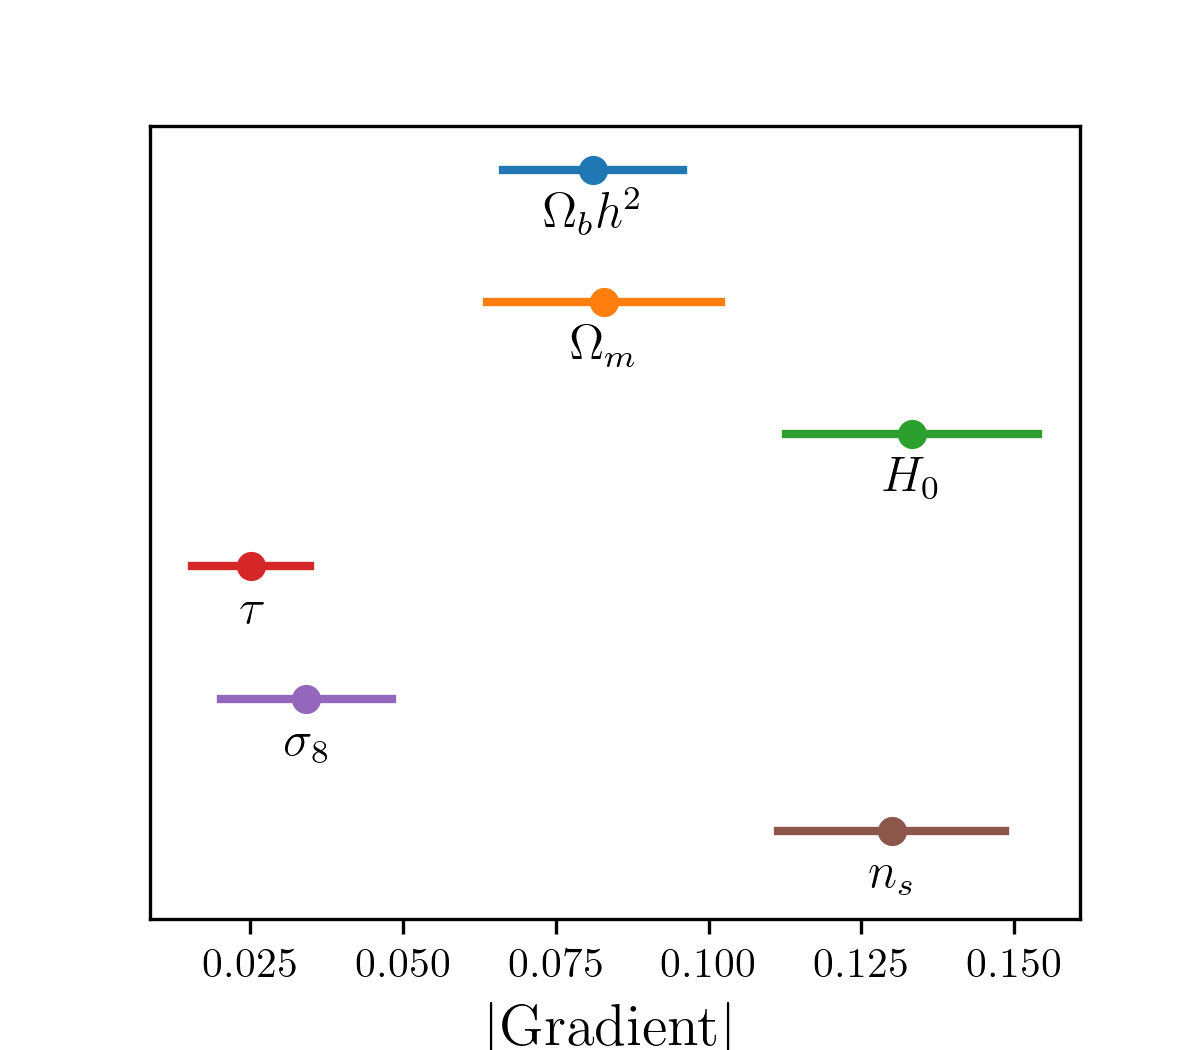
\includegraphics[width=0.8\columnwidth]{../plots/grads.png}
    \centering
    \caption{Measured absolute gradient of the tension coordinate $t$ with respect to each parameter across all data points of both datasets, provided alongside the standard deviation of the measurements}
    \label{fig:grad}
\end{figure}

\begin{figure*}
    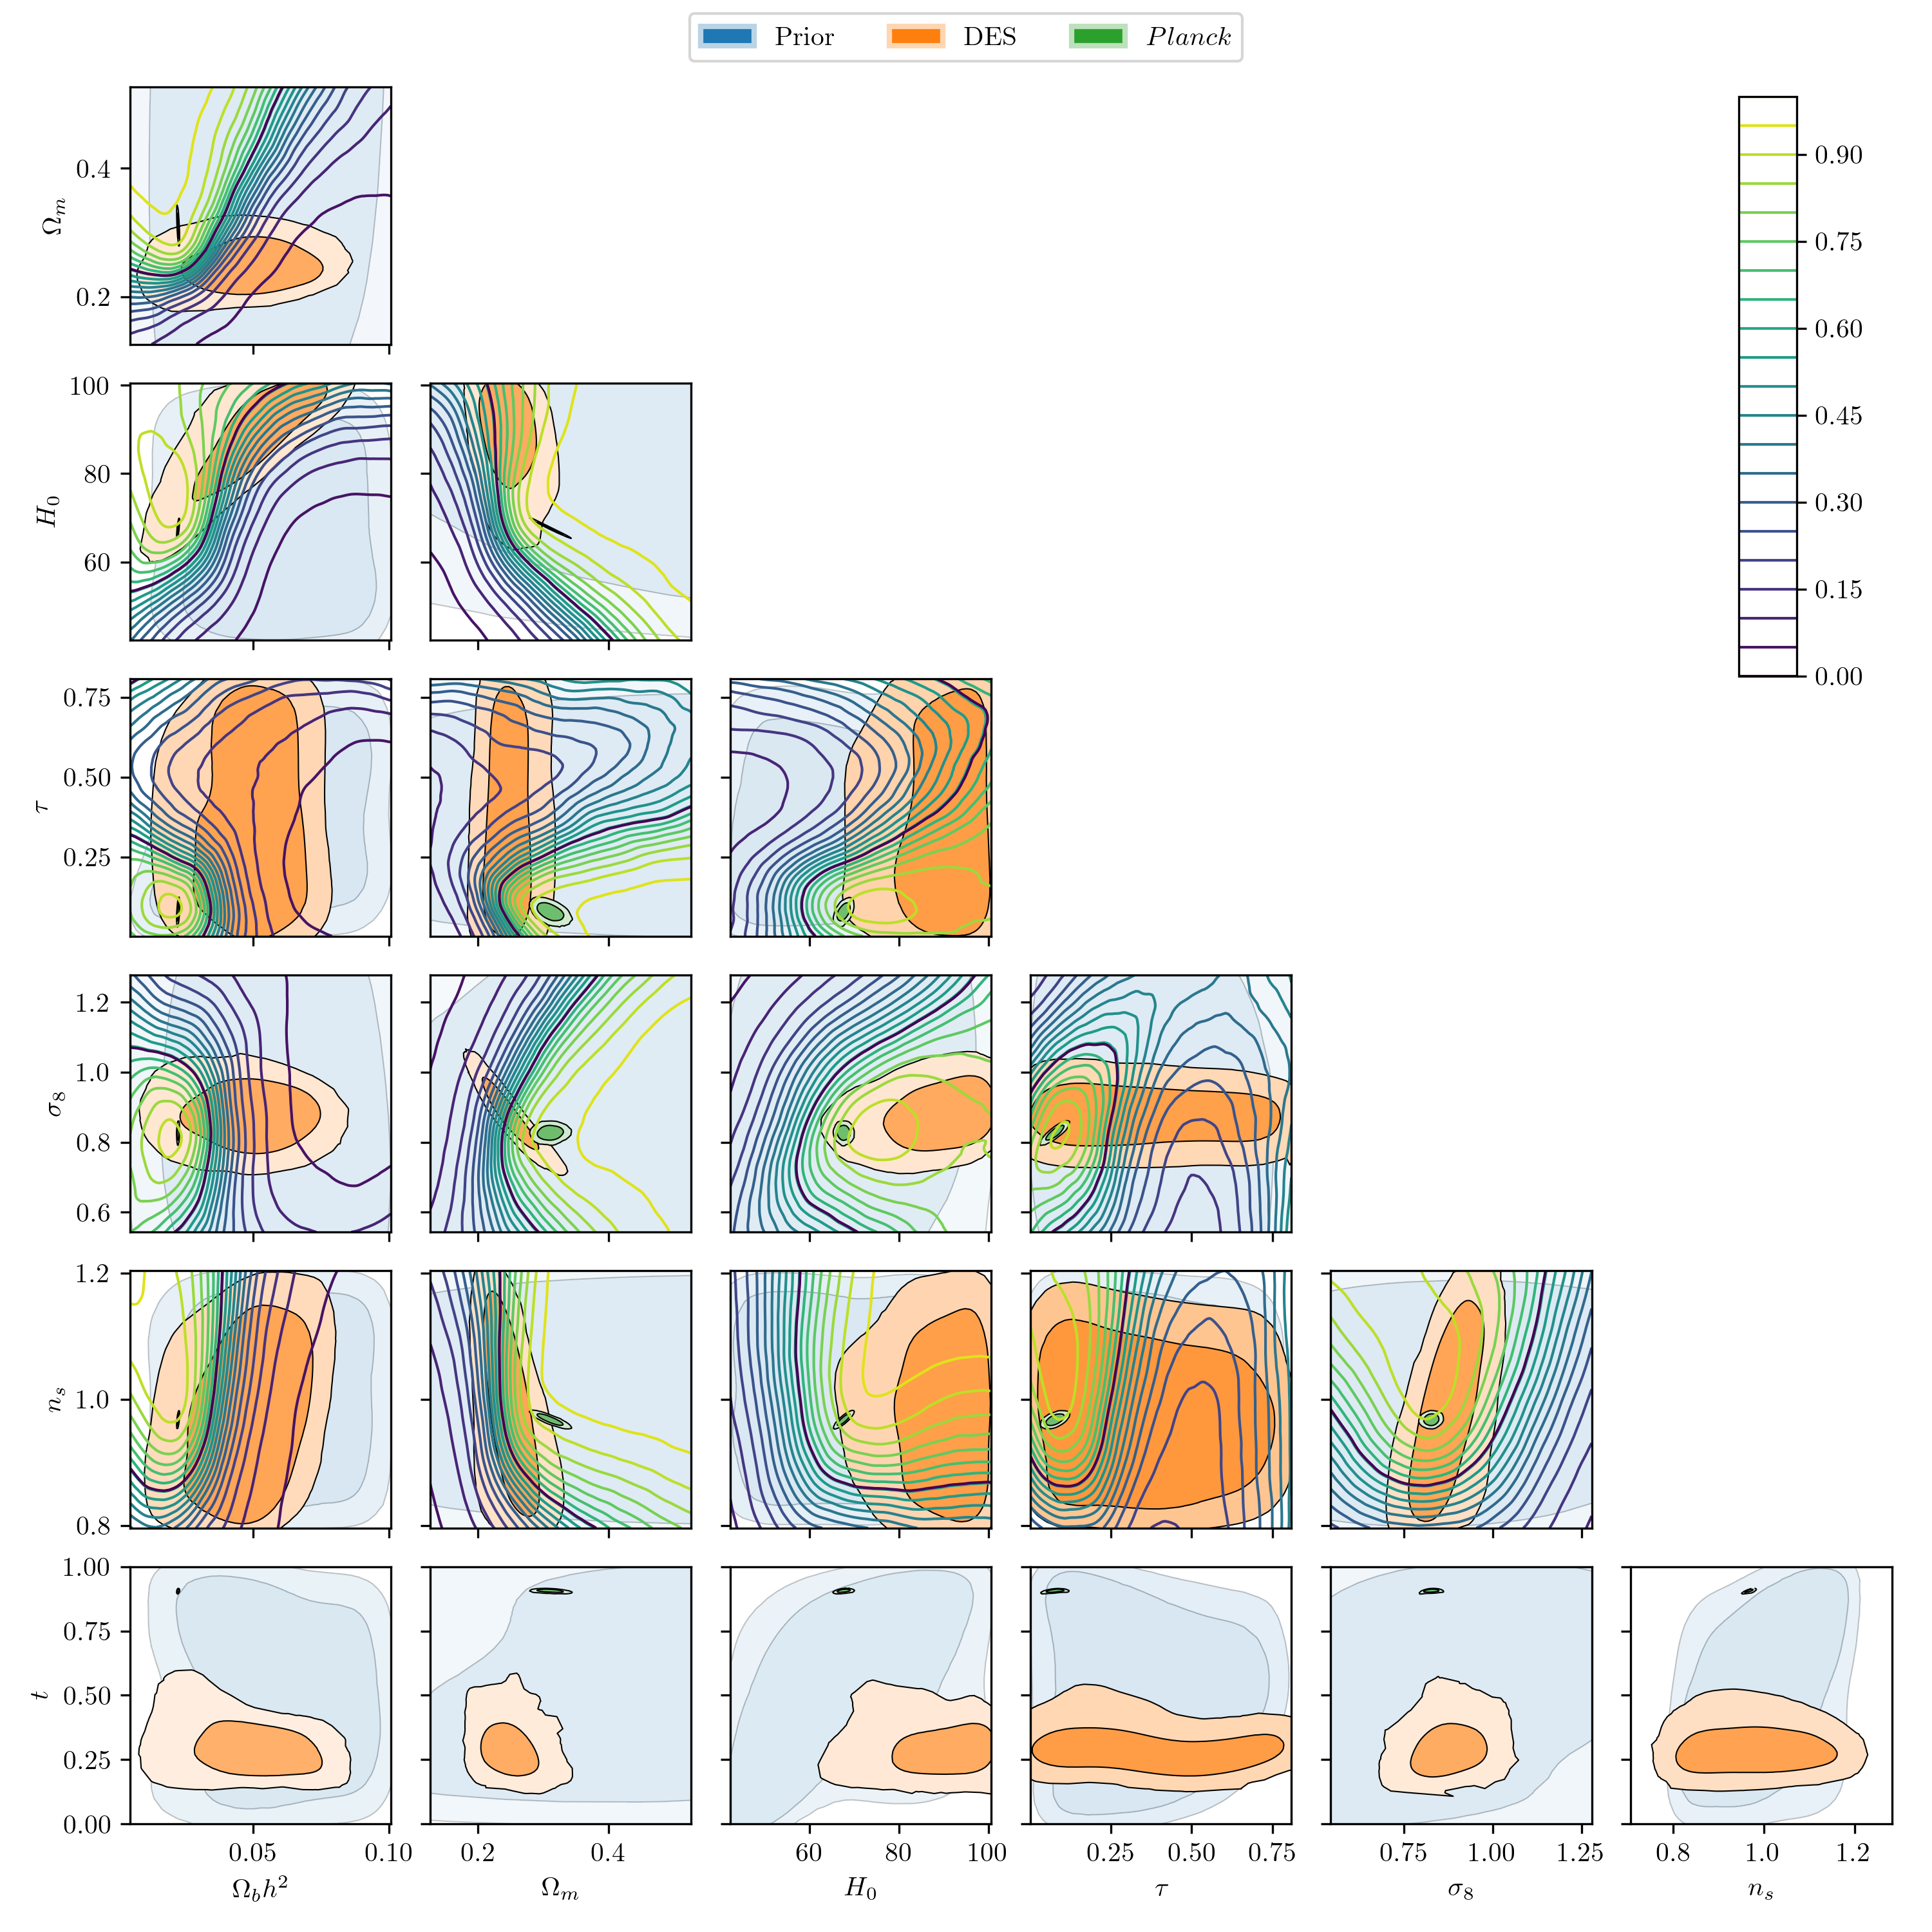
\includegraphics[width=\textwidth]{../plots/six.png}
    \centering
    \caption{The background of these plots shows the two-dimensional marginalised posteriors of the DES and \textit{Planck} datasets, and their shared prior. These posteriors are represented by solid iso-probability contours containing $68\%$ and $95\%$ of the marginalised probability mass. The foreground in these plots, bar the last row, illustrates contour plots of the iso-tension coordinate hypersurfaces. The bold contour line is the midpoint between the two datasets in the 1D tension coordinate. These contour plots are drawn by varying the two relevant cosmological parameters and fixing the other four, then feeding these data points into the trained neural network. The four other parameters are fixed at their respective means in the joint DES-\textit{Planck} dataset. The final row plots the tension coordinate $t$ against the six cosmological parameters, visually emphasising the maximum tension found between these two datasets. The marginalised Bayes factor for this particular optimised neural network is computed to be $-16.9$, while we get an estimate of $\log R_t = -16.8 \pm 0.5$ from 10 separate gradient descent runs on the same neural network setup.}
    \label{fig:six}
\end{figure*}

Before we go further, it is important to reiterate the fact that many local minima exist in our loss function landscape. The many possibilities of a maximum tension coordinate implies that there are potentially a multitude of forms in which the iso-tension coordinate hypersurfaces can be drawn. Fortunately, upon further inspection, we note that the contour plots across all 10 training runs look similar, particularly in the region between the two posteriors. Figure \ref{fig:six} can be said to be representative of all the training runs, however one should still be hesitant in drawing conclusion solely from this figure.

To identify the parameters which contribute most to the six-parameter tension, we calculate the gradient of the tension coordinate with respect to the input parameters. We use \texttt{PyTorch}'s \texttt{torch.autograd} differentiation engine to help us do this, where we obtained the derivative of the tension coordinate with respect to each parameter at each data point. The mean and standard deviation of the absolute gradients for each parameter are plotted in Figure \ref{fig:grad}.

Starting from the top, we find $H_0$ to have the largest gradient, and by extension contribute most to the six-parameter tension. This lends support to the well-established tension of $H_0$ within the cosmology community. It is surprising to see $n_s$ coming in at a close second after the Hubble constant. With the \textit{Planck} posterior falling squarely within the unconstrained DES posterior in the $n_s$ parameter (as inferred from the bottom-rightmost 2D plot in Figure \ref{fig:six}), we would have expected $n_s$ to be one of the least influential parameters. However, the apparent importance of $n_s$ does put a remind us of the aim of the neural network -- to search for non-linear tensions. This result could potentially point to $n_s$ being a significant contributor to the non-linear tension. 

The parameters of $\Omega_b h^2$ and $\Omega_m$ have almost identical absolute gradients, where they both contribute moderately to the six-parameter tension. $\sigma_8$ and $\tau$ bring up the rear, contributing the least to the tension. It is slightly unexpected for the former to be considered less influential, given this parameter is part of the $\Omega_m$ - $\sigma_8$ tension, as discussed in Section \ref{intro}. The apparent insignificance of $\tau$ is more in line with what we would expect, unlike $n_s$, since the DES dataset does not put any constraints on this parameter. 




% \begin{table*}
% \begin{ruledtabular}
% \begin{tabular}{lrrrr}
%     Parameter & $\log R_t$ & $\log S$ & $p$ value & Tension \\
%     \colrule
%     $\Omega_b h^2$  & $1.45 \pm 0.33$ & $1.37 \pm 0.26$ & $(87 \pm 9)\%$ & $(0.17 \pm 0.11)\sigma$ \\
%     $\tau$          & $1.55 \pm 0.15$ & $1.15 \pm 0.06$ & $(79 \pm 2)\%$ & $(0.26 \pm 0.03)\sigma$ \\
%     $\Omega_m$      & $0.43 \pm 0.18$ & $0.47 \pm 0.21$ & $(55 \pm 7)\%$ & $(0.60 \pm 0.10)\sigma$ \\
%     $n_s$           & $-0.18 \pm 0.19$ & $-0.56 \pm 0.26$ & $(27 \pm 5)\%$ & $(1.09 \pm 0.12)\sigma$ \\
%     $\sigma_8$      & $-0.70 \pm 0.29$ & $-1.41 \pm 0.34$ & $(15 \pm 4)\%$ & $(1.45 \pm 0.14)\sigma$ \\
%     $H_0$           & $-0.98 \pm 0.26$ & $-1.56 \pm 0.28$ & $(13 \pm 3)\%$ & $(1.51 \pm 0.11)\sigma$ \\
% \end{tabular}
% \end{ruledtabular}
% \caption{Marginalised Bayes factors from using a dataset containing a single shuffled parameter as input to a trained neural network with six input nodes, as detailed in Section \ref{section:six}. The more positive the $\log R_t$, the more influential the parameter is to defining the tension coordinate.}
% \label{*:shuffled}
% \end{table*}



\subsection{Pair-wise Comparison} \label{section:pair}

We train our neural network for 500 epochs with parameter pairs as the input, and maintain a learning rate of $10^{-4}$ with the Adam optimiser. We perform 10 training repetitions for each parameter pair. The results are given in Table \ref{table:pairwise}, and pairwise contour plots are drawn in Figure \ref{fig:pairs}. It is important to note here that there is a nuanced distinction between the results of this section and the previous section. Here, we seek for parameters \textit{containing} the most tension via parameter pairs, whilst in the previous section we attempted to identify parameters which \textit{contributed} most to the tension in the six-dimensional parameter space.

\begin{table*}
\begin{ruledtabular}
\begin{tabular}{l r r r r}
    Parameter pair & $\log R_t$ & $\log S$ & $p$ value & tension \\
    \colrule
    $H_0$ - $n_s$               &	$-3.18 \pm 0.28$ & $-4.42 \pm 0.31$ & $(0.90 \pm 0.21)\%$ & $(2.61 \pm 0.08)\sigma$ \\
    $H_0$ - $\tau$              &	$-3.54 \pm 0.04$ & $-4.80 \pm 0.07$ & $(0.95 \pm 0.10)\%$ & $(2.59 \pm 0.03)\sigma$ \\
    $\Omega_b h^2$ - $\sigma_8$ &	$-3.04 \pm 0.16$ & $-4.49 \pm 0.21$ & $(1.06 \pm 0.24)\%$ & $(2.56 \pm 0.08)\sigma$ \\
    $\Omega_b h^2$ - $H_0$      &	$-3.25 \pm 0.12$ & $-4.65 \pm 0.10$ & $(1.09 \pm 0.15)\%$ & $(2.55 \pm 0.05)\sigma$ \\
    $\Omega_b h^2$ - $\Omega_m$ &	$-3.35 \pm 0.22$ & $-4.30 \pm 0.14$ & $(1.21 \pm 0.15)\%$ & $(2.51 \pm 0.04)\sigma$ \\
    $\Omega_m$ - $\tau$         &	$-3.16 \pm 0.13$ & $-4.06 \pm 0.06$ & $(1.66 \pm 0.08)\%$ & $(2.40 \pm 0.02)\sigma$ \\
    $H_0$ - $\sigma_8$          &	$-3.09 \pm 0.13$ & $-4.01 \pm 0.04$ & $(1.73 \pm 0.11)\%$ & $(2.38 \pm 0.02)\sigma$ \\
    $\Omega_m$ - $n_s$          &	$-2.17 \pm 0.43$ & $-3.24 \pm 0.45$ & $(1.85 \pm 0.82)\%$ & $(2.36 \pm 0.16)\sigma$ \\
    $\Omega_m$ - $H_0$          &	$-2.79 \pm 0.23$ & $-3.61 \pm 0.13$ & $(2.53 \pm 0.38)\%$ & $(2.24 \pm 0.06)\sigma$ \\
    $\tau$ - $\sigma_8$         &	$-1.82 \pm 0.26$ & $-3.25 \pm 0.28$ & $(2.81 \pm 0.32)\%$ & $(2.20 \pm 0.05)\sigma$ \\
    $\sigma_8$ - $n_s$          &	$-1.82 \pm 0.05$ & $-3.22 \pm 0.13$ & $(3.62 \pm 0.62)\%$ & $(2.09 \pm 0.07)\sigma$ \\
    $\Omega_b h^2$ - $\tau$     &	$-2.41 \pm 0.25$ & $-2.86 \pm 0.19$ & $(3.95 \pm 0.47)\%$ & $(2.06 \pm 0.05)\sigma$ \\
    $\Omega_m$ - $\sigma_8$     &	$-2.25 \pm 0.21$ & $-2.93 \pm 0.31$ & $(4.46 \pm 1.48)\%$ & $(2.01 \pm 0.14)\sigma$ \\
    $\Omega_b h^2$ - $n_s$      &	$-1.85 \pm 0.22$ & $-2.21 \pm 0.35$ & $(5.00 \pm 0.94)\%$ & $(1.96 \pm 0.08)\sigma$ \\
    $\tau$ - $n_s$              &	$-0.67 \pm 0.03$ & $1.57 \pm 0.05$ & $(92.09 \pm 2.84)\%$ & $(0.10 \pm 0.04)\sigma$ \\
    % \hline \hline
\end{tabular}
\rule{0pt}{5pt}
\begin{tabular}{l r r r r}
    Parameter & Mean $\log R_t$ & Mean $\log S$ & Mean $p$ value & Mean tension \\
    \colrule
    $H_0$           & $-3.17 \pm 0.16$ & $-4.30 \pm 0.13$ & $(1.44 \pm 0.19)\%$ & $(2.47 \pm 0.05)\sigma$ \\
    $\Omega_b h^2$  & $-2.78 \pm 0.19$ & $-3.70 \pm 0.20$ & $(2.46 \pm 0.39)\%$ & $(2.33 \pm 0.06)\sigma$ \\
    $\Omega_m$      & $-2.74 \pm 0.24$ & $-3.63 \pm 0.22$ & $(2.34 \pm 0.58)\%$ & $(2.30 \pm 0.08)\sigma$ \\
    $\sigma_8$      & $-2.40 \pm 0.16$ & $-3.58 \pm 0.19$ & $(2.74 \pm 0.55)\%$ & $(2.25 \pm 0.07)\sigma$ \\
    $\tau$          & $-2.32 \pm 0.14$ & $-2.68 \pm 0.13$ & $(20.29 \pm 0.76)\%$ & $(1.87 \pm 0.04)\sigma$ \\
    $n_s$           & $-1.94 \pm 0.20$ & $-2.30 \pm 0.26$ & $(20.69 \pm 1.09)\%$ & $(1.82 \pm 0.09)\sigma$ \\

\end{tabular}
\end{ruledtabular}
    
\caption{The upper table details the quantities of tension calculated from trained neural networks with parameter pairs as its input. The pairs are ordered in decreasing tension. The lower table gives the mean of the quantities of tension from the upper table for each parameter, where the mean is over the pairs which contain the respective parameter. The parameters are also ordered in decreasing tension.}
\label{table:pairwise}
\end{table*}

\begin{figure*}
    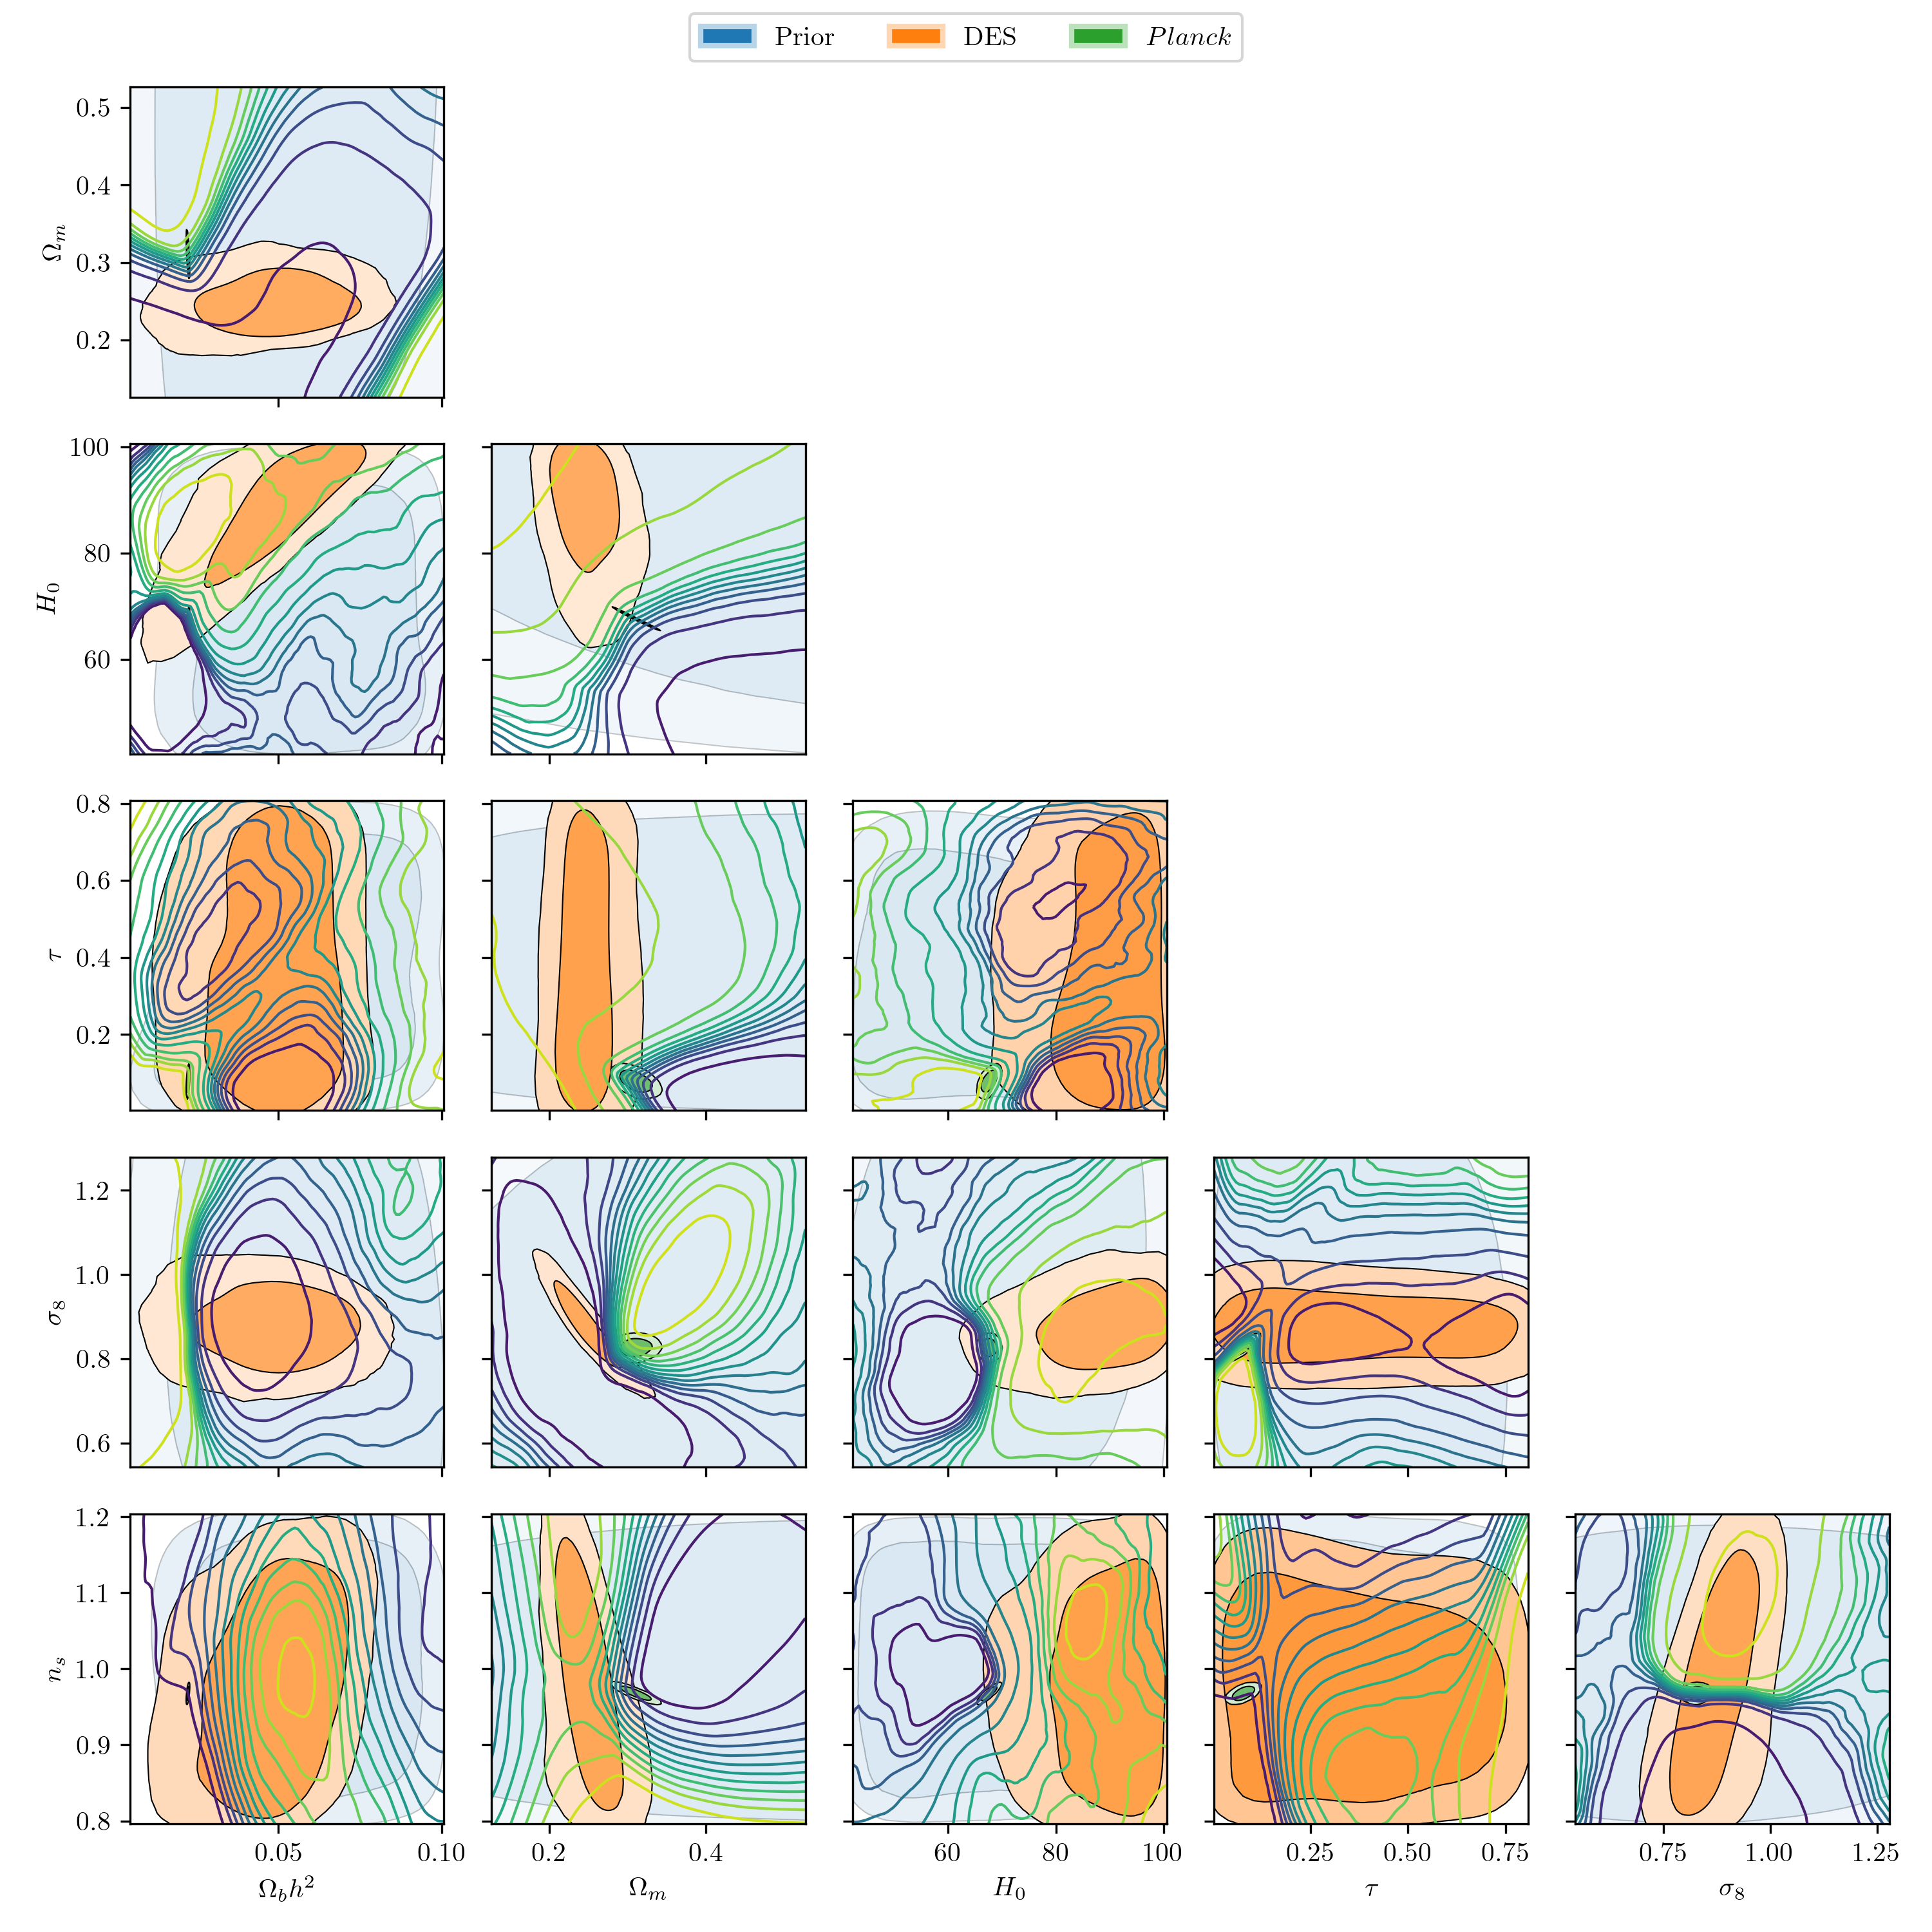
\includegraphics[width=\textwidth]{../plots/pairs.png}
    \centering
    \caption{Similar to Figure \ref{fig:six}, the background shows 2D marginalised distributions of the two datasets and the prior, and the foreground illustrates iso-tension coordinate contour plots. The key difference in this figure is that each plot represents an independent neural network with the respective parameter pair as its input. It is unlike Figure \ref{fig:six}, where all the plots collectively represent a single neural network which takes in all six parameters as its input. Note that the contour plots here are much noisier, particularly in regions that are further away from the two datasets. This likely points to an oversized hidden layer of the neural network, where it begins to over-fit to the statistical noise of the two datasets.}
    \label{fig:pairs}
\end{figure*}

The outcome here generally correlates well with the results from the previous section in terms of the parameter importance. We find $H_0$ to again contain the most tension by a considerable margin, with a mean two-parameter tension of $(2.47 \pm 0.08)\sigma$. We now have three parameters -- $\Omega_b h^2$, $\Omega_m$ and $\sigma_8$, rather than two, containing similar moderate tension. However, the largest difference with our previous result is the ranking of $n_s$ -- the parameter has dropped from second place to last and is now considered to contain the least tension. The contrast in results could potentially point to $n_s$ being a more significant contributor to non-linear tensions in high-dimensional parameter spce, but less able to influence the tension coordinate in lower dimensions.

Looking at the ranking of parameter pairs, it is interesting to note that $\Omega_m$ - $\sigma_8$ is ranked as the 3rd least discrepant pair with a marginalised tension of around $2\sigma$. This is considerably less than the well-known $3\sigma$ tension calculated in two dimensions. It appears that by considering non-linear tension coordinates, more tension can be found in other pairs of parameters, particularly those that consist of either $H_0$ or $\Omega_b h^2$.


\section{Conclusions}

In this paper, we have constructed a basic functioning neural network with an appropriate loss function, in the form of the Bayes factor, to seek out non-linear cosmological tensions. We applied this neural network to the six parameters of $\Omega_b h^2$, $\Omega_m$, $H_0$, $\tau$, $\sigma_8$ and $n_s$ from the DES and \textit{Planck} datasets, and were able to isolate a non-linear tension of $(5.47 \pm 0.08)\sigma$ -- a discrepancy surpassing the $5\sigma$ gold standard of scientific discovery.

We identified the source of tension between the DES and \textit{Planck} datasets via two methods -- the first uses the gradient of the tension coordinate with respect to the cosmological parameters, and the second compares the tension found in pairs of parameters. We found the Hubble constant $H_0$ to be the largest \textit{contributor} to the six-parameter tension, and also the parameter \textit{containing} the most tension, both by considerable margins. 

This result pinpoints the constraints of the Hubble constant $H_0$ to be the key source of discrepancy between the DES and \textit{Planck} datasets. The weak lensing tension of the $\Omega_m$ - $\sigma_8$ pair discussed in Section \ref{intro} was surprisingly one of the parameter pairs which contained the least non-linear tension. This could be an indication of the weak lensing tension being a manifestation of the Hubble tension rather than an intrinsic tension within $\Omega_m$ - $\sigma_8$, especially given these are derived parameters which are not independent.

A surprising observation in our results shows the $n_s$ parameter as a significant contributor to the non-linear six-parameter tension, but does not contain much tension in itself. The unconstrained $n_s$ posterior of the DES dataset should have meant that $n_s$ does not have a large influence on the high dimensional tension, but the outcome of our first method shows otherwise. Given the unexpected nature of this result, it is important that more work is done in this area to either support or disfavour this peculiar observation.


\begin{acknowledgments}
I am deeply grateful to Dr. Will Handley for offering his unwavering support, guidance and expertise at every stage of this project.
\end{acknowledgments}

% \appendix
% \section{Appendixes}
% \section{A little more on appendixes}
% \subsection{\label{app:subsec}A subsection in an appendix}




% The \nocite command causes all entries in a bibliography to be printed out
% whether or not they are actually referenced in the text. This is appropriate
% for the sample file to show the different styles of references, but authors
% most likely will not want to use it.

\bibliography{apssamp}% Produces the bibliography via BibTeX.

\end{document}
%
% ****** End of file apssamp.tex ******